\documentclass[12pt,openany]{jreport}
\usepackage{float}
\usepackage{listings}
\usepackage{bezier}
% \usepackage[dvipdfmx]{graphicx}
\usepackage{sotsuron}
\usepackage{misc}
\usepackage{verbatim}
\usepackage{listings}
\usepackage{ascmac}
\usepackage{amsmath}
\usepackage{cite}
\usepackage{siunitx} %%SI単位系用
\usepackage{graphicx}
\usepackage[dvipdfmx]{color}
\usepackage{breqn}
\usepackage{xcolor}
\usepackage{url}

\lstset{
  language={bash},
  basicstyle={\ttfamily},
  identifierstyle={\small\ttfamily},
  keywordstyle={\ttfamily\small\bfseries\color[rgb]{0,0,1}},
  ndkeywordstyle={\ttfamily\small},
  stringstyle={\small\ttfamily\color[rgb]{1,0,1}},
  frame={tb},
  breaklines=true,
  columns=[l]{fullflexible},
  xrightmargin=0zw,
  xleftmargin=3zw,
  numberstyle={\scriptsize},
  numbersep=1zw,
  lineskip=-0.5ex,
  showstringspaces=false
}
\renewcommand{\lstlistingname}{リスト}
\newcommand{\myfrac}[2]{\frac{\,{#1}\,}{\,{#2}\,}}

\renewcommand{\baselinestretch}{1.2}

\begin{document}
\begin{titlepage}
\centering
{\Huge\bf 学位論文} \\
\vspace{3.0cm}

{\LARGE
太陽光発電データの時刻補正手法とElasticsearchノードのクラスタ化手法の提案                        \\[4.0mm]%ここにタイトルをいれてね

\vspace{1.5cm}

\hspace{1.0mm}
\begin{tabular}{ll}

           &                            \\
提出年月日 & \ 令和 6 年 1 月 31 日    \\
% 改訂日 & \ 令和  年  月  日    \\
           &                            \\
           &                            \\
指導教員   & \ 都築\quad 伸二\quad 教授  \\
           &                            \\
           &                            \\           
入学年度   & \quad 令和 4年             \\
学科名     & \quad 電子情報工学専攻       \\           
論文提出者 & \quad 祖父江  \    匠真    \\
\end{tabular}
}
\end{titlepage}
        % 卒論の表紙です
\pagestyle{headings}
\pagenumbering{Roman}
\chapter*{内容梗概}
\addcontentsline{toc}{chapter}{内容梗概}

本論文は,筆者が愛媛大学大学院理工学研究科電子情報工学専攻電気電子工学コースに在学中に
行った, 太陽光発電データの時刻補正手法とElasticsearchノードのクラスタ化手法の提案についてまとめたものであり, 以下の5章から構成されている.\\

\begin{quote}
      \begin{description}

            \item[第\ref{chap:first}章 緒論]\ \\
            本研究を行うに至った経緯及び, 本研究の目的について述べている.
            \vspace{3.0mm}
            
            \item[第\ref{chap:second}章 太陽光発電データの時刻補正手法]\ \\
            ここでは, 太陽光発電データの計測時刻の補正手法を提案する. また, pvlibと呼ばれる太陽光発電シュミレーターライブラリを導入して, 計測データを前処理することによる補正誤差の改善手法についても提案する.
            \vspace{3.0mm}
            
            \item[第\ref{chap:third}章 単一Elasticsearchノードをクラスタ化する前に行うデータ移行]\
            ここでは, 単一Elasticsearchノードをクラスタ化する前に行うデータ移行について述べており, CO\textsubscript{2}データの移行とLEAFの運行日誌のデータ移行プロセスを詳述し, 移行後のデータ可視化による確認を行っている.
            \vspace{3.0mm}
            
            \item[第\ref{chap:fourth}章 仮想環境を使用したクラスタリング動作の検証]\ \\
            ここでは, 仮想環境を使用したクラスタリング動作の検証について述べており, バージョンの異なるElasticsearchノードを用いたクラスタ構築の可否や, 既存Elasticsearchノードの異なるクラスタへの参加の可否の検証結果について述べる.
            \vspace{3.0mm}
            
            \item[第\ref{chap:fifth}章 結論と今後の課題]\ \\
            本研究によって明らかになった事項や今後の研究課題についてまとめている.
      \end{description}
\end{quote}
   % 内容梗概
\clearpage
\tableofcontents          % 目次が勝手に生成されます%
\clearpage
\pagestyle{headings}
\pagenumbering{roman}
\pagestyle{headings}
\pagenumbering{arabic}
\chapter{緒論}
\label{chap:first}

%%序論を書いてください. 卒論の内容を簡単にまとめてください. 
太陽光発電は, 再生可能エネルギー源として世界中で注目されており, 効率的な運用と管理には正確な計測データが不可欠である. しかしながら, 通信システム工学研究室で管理している太陽光発電データは, データを計測しているPCの内部時計が標準時刻とずれているため, 他地点で計測しているデータと時刻同期ができない問題があった.

本論文では, この問題に対処するため, 太陽光発電データの計測時刻の補正手法を提案する. また, pvlibと呼ばれる太陽光発電シュミレーターライブラリを導入して, 計測データを前処理することによる補正誤差の改善手法についても提案する.
次に, 発電データ等を蓄積しているElasticsearchサーバをクラスタ化して故障耐性を向上する際に必要な作業の実施方法を提案する. 単一で動いているサーバのデータをクラスタ化サーバにするためのプロセスについて提案する. バージョンの異なるElasticsearchノードを用いたクラスタ構築の可否や, 既存Elasticsearchノードの異なるクラスタへの参加の可否の検証結果も述べる. 

本論文は以下の構成となっている. 第2章では, 太陽光発電データの計測時刻を標準時に補正するために, 理論値との相互相関を用いる手法を提案する. 第3章では, 単一で動いているサーバのデータをクラスタ化するためのデータ移行手法について提案する. 第4章では, バージョンの異なるElasticsearchノードを用いたクラスタ構築の可否や, 既存Elasticsearchノードの異なるクラスタへの参加の可否の検証結果も述べる. 第5章では, 本研究の成果と課題を明らかにする.   % 緒論

\chapter{太陽光発電データの時刻補正手法}
\label{chap:second}

\section{緒言}
本章では, 太陽光発電データの計測日時の補正手法を提案する.

% 20220523

\section{太陽光発電の計測データの問題点について}
本研究で管理している太陽光発電データは, データを計測しているPCの内部時計が標準時刻とずれているため, 他地点で計測しているデータと時刻同期ができない問題があった. 

そこで, 時刻がずれていない実測データと, 計算式により求まる大気外日射量との間の時間的遅延の秒数を相互相関を用いて求めることで, 実測データを標準時に補正する.

\section{大気外日射量の計算式}
任意の緯度経度, 日時における大気外日射量$Q$は, 任意の緯度$\phi$, 経度$\lambda$の地点における任意の日時, 太陽高度$\alpha$から求めることができる.

まず, 次式より元旦からの通し日数$dn$に基いて定めた$\theta$を用いて, 当該日の太陽赤緯$\delta$, 地心太陽距離$\frac{r}{r^{*}}$, 均時差$E_q$をそれぞれ以下の式により求める.
\begin{eqnarray}
  \theta =  \frac{2\pi (dn-1)}{365}
\end{eqnarray}

\begin{eqnarray}
  \begin{split}
    \delta =  0.006918-0.399912\cos \theta+0.070257\sin \theta-0.006758\cos 2\theta\\
    +0.000907\sin 2\theta-0.002697\cos 3\theta+0.001480\sin 3\theta
  \end{split}
\end{eqnarray}

\begin{dmath}
  \frac{r}{r^{*}} =  \frac{1}{\sqrt{1.000110+0.034221\cos \theta+0.001280\sin \theta+0.000719\cos 2\theta+0.000077\sin 2\theta}}
\end{dmath}

\begin{eqnarray}
  \begin{split}
    E_q =  0.000075+0.001868\cos \theta-0.032077\sin \theta\\
    -0.014615\cos 2\theta-0.040849\sin 2\theta
  \end{split}
\end{eqnarray}

日本標準時間から, 太陽の時角$h$を求める.

\begin{eqnarray}
  h = \frac{(日本標準時間-12)\pi}{12}+標準子午線からの経度差+E_q
\end{eqnarray}

$\delta$, $\phi$, $h$の値が既知となったので$\alpha$は

\begin{eqnarray}
  \alpha = \arcsin (\sin \phi\sin \delta+\cos \phi\cos \delta\cos h)
\end{eqnarray}

により求まる.

最後に, $Q$が

\begin{eqnarray}
  Q = 1367(\frac{r^{*}}{r})^{2}\sin \alpha
\end{eqnarray}

により求まる. 1367\si{\watt}/\si{\metre\squared}は太陽定数である.

式(2.1)~式(2.7)を用いることで, 任意の緯度経度, 日時における大気外日射量が求まる.

% 20220529

\subsection{実測データと大気外日射量との比較}
Elasticsearchサーバーから取得した2022年6月2日の実測データと, 計算式から求めた大気外日射量をプロットしたものを図\ref{20220529-p1}に示す. 実測データは地表に設置された太陽光パネルが計測したものであるのに対して, 大気外日射量は地球大気の上端(約8km上空)で受け取る日射量を計算したものであるため, 一日を通して最大となる日射量の大きさに差がある.

\begin{figure}[H]
  \begin{center}
    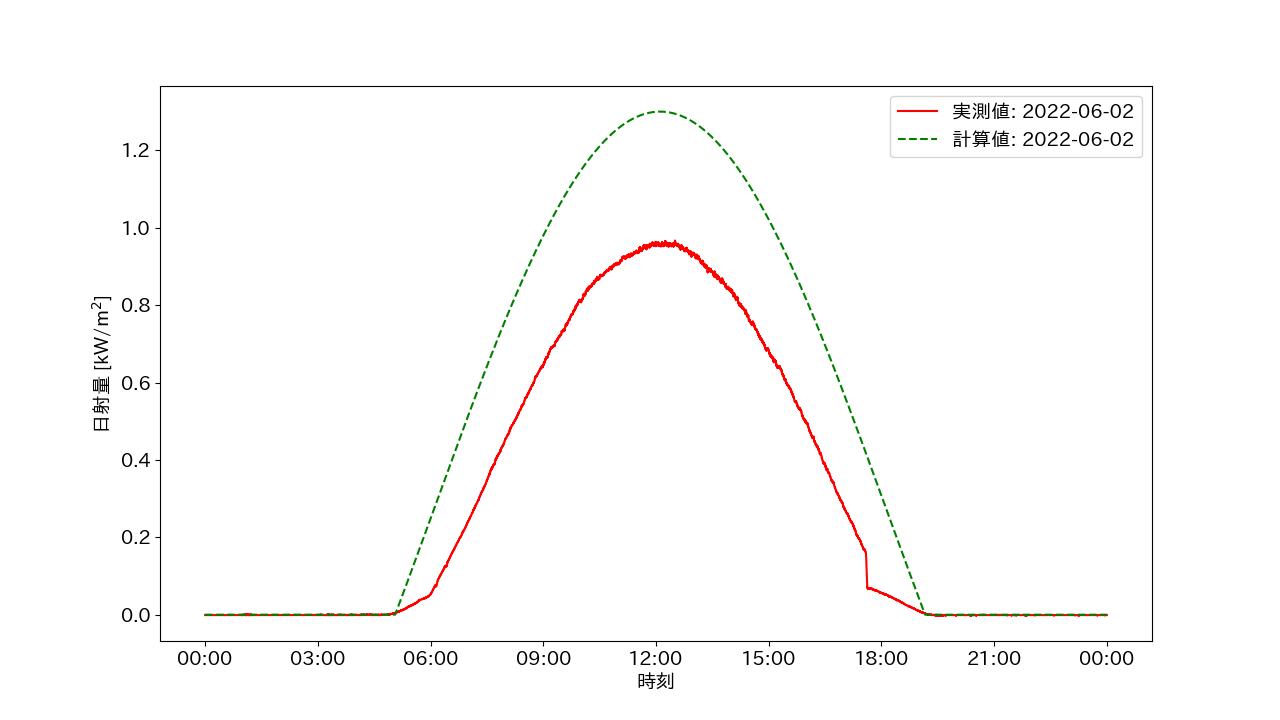
\includegraphics[width=160mm]{sotu/figure/2/original-20220602-corr.png}
    \caption{2022年6月2日の日射量の実測データと大気外日射量をプロットしたもの}
    \label{20220529-p1}
  \end{center}
\end{figure}

% 20220620

\subsection{相互相関による時刻補正法}
今回, 相互相関の計算に使用する期間を, 2022年6月2日0時0分から2022年6月2日23時59分までとする.

% 2022年6月2日を選定した理由は, 図\ref{20220529-p1}より, 2022年6月2日の実測データの概形は大気外日射量の概形と類似していたためである.

相互相関の計算に使用する実測データの計測日時から大気外日射量を求め, 実測データとの相互相関を計算する.

相互相関を計算した結果, 実測データを124秒遅らせた際に, 相関が最大となった.

今回使用した実測データには計測日時のずれは殆どないため, 実測データを遅らせていない際に相関が最大となるのが正しい.

これは, 相互相関を計算する際に地表日射量ではなく大気外日射量を使用していることが原因であると考えられる.

\section{地表日射量の予測}

地表日射量の予測を行うため, 式(2.1)~式(2.7)を使った方法ではなく, pvlibライブラリを使用して地表日射量を求め, 相互相関を計算する.

\subsection{pvlibの概要}
pvlibは, 太陽光発電システムの性能シミュレーションや関連するタスクを実行するための関数とクラスのセットを提供するライブラリである. 

以下は, pvlibの主な特徴である.

\begin{itemize}
  \item 太陽位置計算: pvlibは, 地球上の任意の場所における太陽の位置を計算する機能を提供する. これは, 太陽の方位角や高度角を求めるのに使用される.
  \item 大気透過モデル: 大気を通過する太陽放射の量や質を推定するモデルが含まれている.
  \item 太陽光発電システムの性能モデリング: 太陽光発電モジュールやインバーターの性能モデルが含まれており, 異なる条件下での太陽光発電システムの出力をシミュレートできる.
\end{itemize}

\subsection{実測データとpvlibにより求まる地表日射量の比較}
Elasticsearchサーバーから取得した実測データと, pvlibを用いて求めた地表日射量をプロットしたものを図\ref{2-p1}に示す.
% 図\ref{2-p1}はElasticsearchサーバーから取得した2022年6月2日の日射量データと, リサイクル館の緯度経度と日付情報を入力としてpvlibより求めた地表日射量をプロットしている.

図\ref{2-p1}と図\ref{20220529-p1}と比較すると, 大気外日射量より地表日射量の方が実測データにより近い概形となっていることが分かる.

\begin{figure}[H]
  \begin{center}
    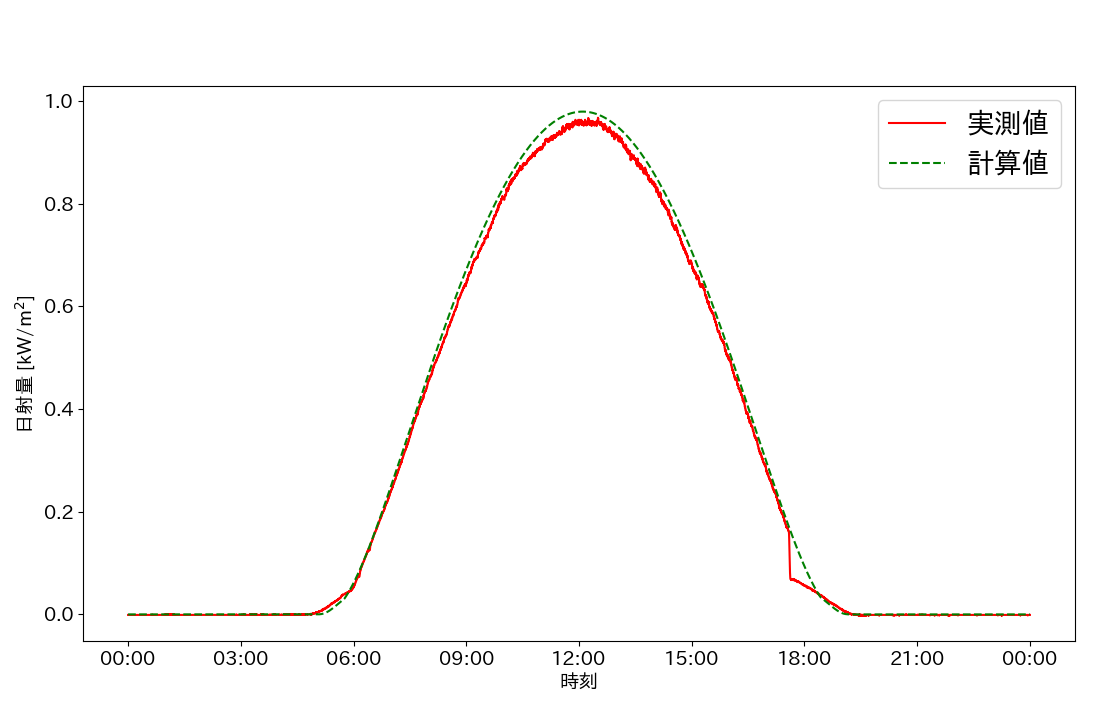
\includegraphics[width=160mm]{sotu/figure/2/pvlib-20220602-corr.png}
    \caption{2022年6月2日の実測データと地表日射量をプロットしたもの}
    \label{2-p1}
  \end{center}
\end{figure}

\subsection{地表日射量との相互相関による時刻補正法}
今回, 相互相関の計算に使用する期間を, 2022年6月2日0時0分から2022年6月2日23時59分までとする.

実測データの計測日時から地表日射量を求め, これらの値から相互相関を計算する.

相互相関を求めた結果, 実測データ74秒遅らせた際に, 相関が最大となることが分かった.

式(2.1)~式(2.7)より求めた大気外日射量を用いて相互相関を計算した時と比較して, 124秒から74秒へと50秒改善した.

\section{前処理の追加による時刻補正法とその精度}

図\ref{2-p1}では, 日没の辺りにおいて, 実測データと地表日射量の概形が大きく異なっている.

太陽光パネルの周囲にある建造物や, 天候といった外部要因による実測データのひずみを事前に取り除いた上で相互相関を計算することで, 相互相関の計算結果が改善するか検証する. そこで, 実測データに対して前処理を追加する.

前処理を含めた相互相関の計算方法は以下の手順で行う.

\begin{enumerate}
  \item 実測データの日射量を0 \si{\kilo\watt}/\si{\metre\squared}と見なすしきい値の指定: まず, 実測データをフィルタリングするために日射量のしきい値を設定する. 今回は, 0.2 \si{\kilo\watt}/\si{\metre\squared}をしきい値として設定する.
  \item しきい値に該当する計測日時の特定: 続いて, 実測データの各データ点から0.2 \si{\kilo\watt}/\si{\metre\squared}を減算して絶対値を取った際に最も0に近い値を取る計測日時を午前と午後でそれぞれ一点ずつ特定する.
  \item 特定した計測日時を使った実測データのフィルタリング: 前のステップで得た計測日時を使用して, 2点の計測日時の外側にある実測データの日射量を0 \si{\kilo\watt}/\si{\metre\squared}とする.
  \item 地表日射量との相互相関の計算: 実測データをフィルタリングした後, 地表日射量との相互相関を計算する.
\end{enumerate}

図\ref{2-p2}に, 上述の前処理を行った実測データと, 地表日射量をプロットしたものを示す.

\begin{figure}[H]
  \begin{center}
    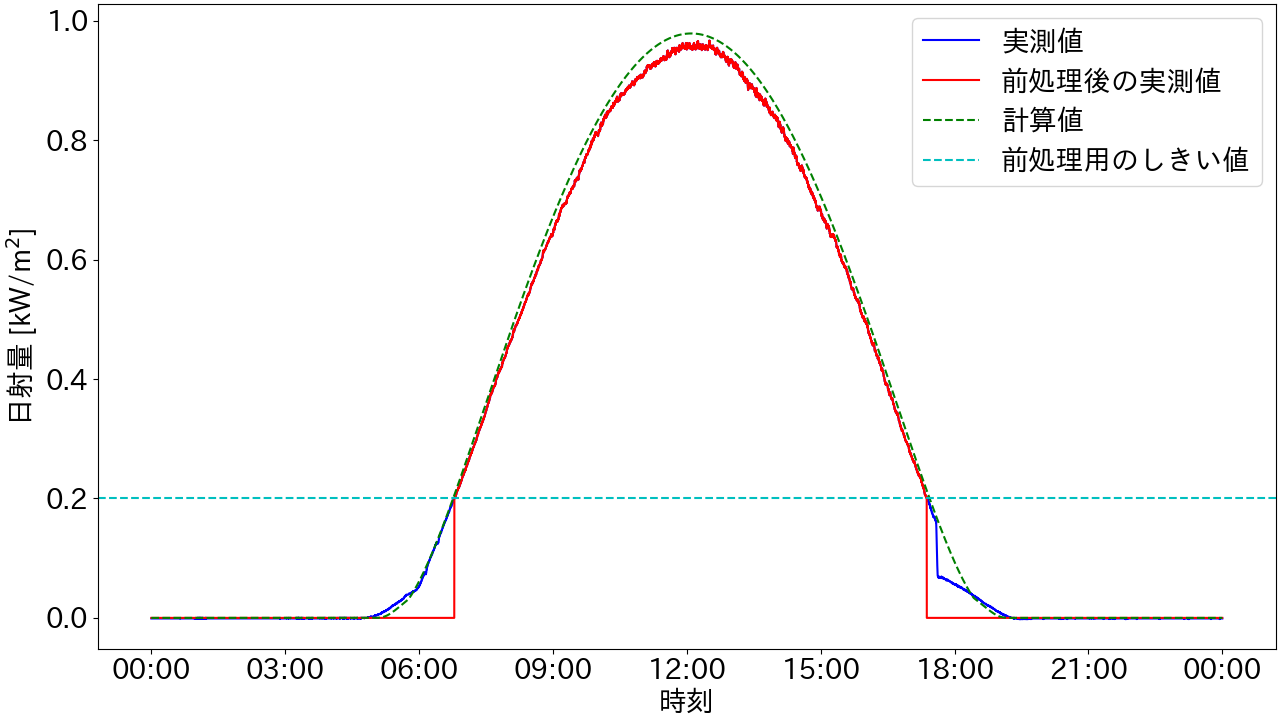
\includegraphics[width=140mm]{sotu/figure/2/drop-under-0.2-q.png}
    \caption{前処理を行った実測データと, 地表日射量をプロットしたもの}
    \label{2-p2}
  \end{center}
\end{figure}

前処理を行った実測データと, 地表日射量から相互相関を計算した結果, 実測データを27秒遅らせた際に, 相関が最大となった.

前処理を追加したことで相互相関の結果が, 74秒から27秒へと47秒改善した.

\section{結言}
本章では太陽光発電データの計測時刻の補正手法を提案した.
次章では学内ゾーンで稼働している Elasticsearch クラスタへのデータ移行について述べる.   % 2章

\chapter{単一Elasticsearchノードをクラスタ化する前に行うデータ移行}
\label{chap:third}

\section{緒言}
本章では単一Elasticsearchノードにあるデータのエクスポート, 重複データの削除, そしてクラスタにインポートするデータ移行に関する作業ついて述べる.

\section{Elasticsearchの概要}
Elasticsearchは, 分散処理に対応した全文検索エンジンである. 主な特徴は, 以下の通りである.

\begin{itemize}
  \item 高速な検索性能: ビッグデータなどの巨大で複雑なデータの集合にも対応可能
  \item 部分一致検索が可能: 検索キーワードの一部に一致するドキュメントも検索可能
  \item ほぼリアルタイムの検索: ドキュメントにインデックスを付けてから検索可能になるまで約1秒程度
  \item スケーラビリティ: サーバー数を増やすことで, 検索性能と処理能力を拡張可能
\end{itemize}

これらの特徴から, Elasticsearchは, 以下のような用途に適している.

\begin{itemize}
  \item ログ分析: Webサイトやアプリケーションのログから, アクセス状況やエラー情報を分析する
  \item セキュリティインテリジェンス: ネットワークやシステムから, セキュリティ脅威を検知する
  \item ビジネス分析: 顧客データや販売データから, トレンドや傾向を分析する
\end{itemize}

\section{Kibanaの概要}

Kibanaは, Elasticsearchに保存されたデータを可視化するためのツールである. 主な特徴は, 以下の通りである.

\begin{itemize}
  \item 直感的な操作性: ドラッグ&ドロップで簡単に可視化を作成できる
  \item 豊富な可視化機能: グラフ, 表, 地図など, さまざまな可視化機能を提供
  \item 高度なフィルタリング機能: 条件を指定して, データを詳細に絞り込むことができる
\end{itemize}

これらの特徴から, Kibanaは, 以下のような用途に適している.

\begin{itemize}
  \item ログ分析: Webサイトやアプリケーションのログから, アクセス状況やエラー情報を可視化する
  \item セキュリティインテリジェンス: ネットワークやシステムから, セキュリティ脅威を可視化する
  \item ビジネス分析: 顧客データや販売データから, トレンドや傾向を可視化する
\end{itemize}

% \section{学内ゾーンで稼働しているElasticsearchシステムの状況}
% 学内ゾーンでは, 単一ノードで稼働する133.71.106.168のElasticsearchと, 133.71.106.170, 133.71.106.141, 133.71.106.136のElasticsearchノードによって構成されたElasticsearchクラスタが稼働している.

% 133.71.106.168のElasticsearchには, CO\textsubscript{2}濃度監視システムによって計測されたデータとLEAFの運行日誌に関するデータが保存されている.

% \section{CO\textsubscript{2}濃度監視システムの概要}
% CO\textsubscript{2}濃度監視システムとは共通講義棟 C, 工学部 5 号館,工学部 4 号館の各講義室(計 24 部屋)の CO2 濃度を学内ネットワーク内の web サイトで閲覧することができるシステムである.

\section{データ移行対象のElasticsearchインデックスについて}

133.71.106.168で稼働している単一ノードのElasticsearchに保存されたCO\textsubscript{2}データとLEAFの運行日誌に関するデータを, Elasticsearchクラスタへ移行する.

\subsection{CO\textsubscript{2}データ}

CO\textsubscript{2}データが保存されたインデックスは, インデックス名にco2という文字列が含まれているため, co2という文字列を含む全てのインデックスを移行対象とした.

\subsection{LEAFの運行日誌に関するデータ}

LEAFの運行日誌に関するデータが保存されたインデックスは以下の2つである.

\begin{itemize}
  \item movement\_diary
  \item movement\_diary01
\end{itemize}

上記のインデックスに保存されているデータについて説明する.

以下にmovement\_diaryとmovement\_diary01のドキュメントの違いを列挙する.

\begin{enumerate}
  \item driverフィールド:
        \begin{itemize}
          \item movement\_diaryのドキュメントでは, driverフィールドは文字列である.
          \item movement\_diary01のドキュメントでは, driverフィールドは配列で, その中に文字列と2つのnull値が含まれている.
        \end{itemize}
        
  \item ``destination''フィールド:
        \begin{itemize}
          \item movement\_diaryのドキュメントでは, ``destination''フィールドは単一の文字列である.
          \item movement\_diary01のドキュメントでは, ``destination''フィールドは配列で, その中に2つの文字列が含まれている.
        \end{itemize}
        
  \item ``charge\_place''フィールド:
        \begin{itemize}
          \item movement\_diaryのドキュメントには, ``charge\_place''フィールドは存在しない.
          \item movement\_diary01のドキュメントでは, ``charge\_place''フィールドが追加されているが, その値は空文字列である.
        \end{itemize}
        
  \item ``battery\_rate''フィールド:
        \begin{itemize}
          \item movement\_diaryのドキュメントには, ``battery\_rate''フィールドは存在しない.
          \item movement\_diary01のドキュメントでは, ``battery\_rate''フィールドが追加されており, その値は数値である.
        \end{itemize}
        
  \item ``battery\_rate\_distance''フィールド:
        \begin{itemize}
          \item movement\_diaryのドキュメントには, ``battery\_rate\_distance''フィールドは存在しない.
          \item movement\_diary01のドキュメントでは, ``battery\_rate\_distance''フィールドが追加されており, その値は数値である.
        \end{itemize}
\end{enumerate}

上述したドキュメントの違いより, movement\_diary01はmovement\_diaryのもつ全ての情報を保持しており, 更にmovement\_diaryにはないフィールドを持っている. 更に, movement\_diaryとmovement\_diary01のドキュメント数は等しく, すべてのドキュメントのタイムスタンプが一致しているため, movement\_diary01インデックスのみ移行した.

\section{CO\textsubscript{2}データの移行手順ついて}
Elasticsearchに保存されたCO\textsubscript{2}データには, 計測時刻, 部屋番号, 部屋の気温, CO\textsubscript{2}濃度などの情報が含まれている.

CO\textsubscript{2}デーのタ移行を行うに当たって, 計測時刻と部屋番号の組み合わせが重複しているデータが一部存在しているため, 重複データを削除した上でデータを移行する必要があった. そこで一度, 移行元のElasticSearchサーバーのデータをローカルマシンにエクスポートして, 重複データを取り除いた上で, 移行先のElasticSearchサーバーにデータをインサートした.

\subsection{データのエクスポート}
移行元のElasticSearchサーバーのデータのローカルマシンへのエクスポートには, elasticdumpライブラリを使用して, JSON形式でエクスポートした.その際, co2という文字列を含むインデックスのデータのみをエクスポートした.

\subsection{データの重複削除}
重複データの削除はインストールが容易だったSQLiteデータベースを用いて行った.

SQLiteは, 軽量で自己完結型のデータベースエンジンである. SQLiteは以下の特徴を持っている.

\begin{itemize}
  \item 軽量: SQLiteは非常に小さく, リソースの少ない環境でも動作する.
  \item 自己完結型: データベースが単一のファイルとして存在し, 外部の依存関係がない.
  \item 
        トランザクション: SQLiteはACIDトランザクションをサポートしており, データの整合性を保つ. 
  \item 
        フリーかつオープンソース: SQLiteはパブリックドメインに属し, 誰でも自由に使用, 変更, 配布可能である.
\end{itemize}

SQLiteでは, 複合主キーを使って複数のテーブルカラムの組み合わせを一意の識別子として扱うことができる. これにより, 同じ組み合わせのデータを重複して挿入しようとした場合, データベースエンジンがコンフリクトエラーを発生させ, 重複データの挿入を阻止する. そのため, 今回の重複データ削除には適していると判断した.

今回使用したSQLiteでは, 部屋番号(number)と計測時刻(utctime)を複合主キーとして設定した. 以下のリスト\ref{sc1}, リスト\ref{sc2}に示すように, 移行元のElasticSearchサーバーに保存されているco2インデックスのドキュメントは, ドキュメントの持つフィールドが統一されておらず, 一部のセンサー情報が存在しないドキュメントが存在する. そのため, SQLiteへのデータ挿入時にコンフリクトエラーが発生した場合は, 既存のレコードと挿入しようとしたレコードを比較し, 既存レコードの値がNULLであるカラムにおいて, 挿入しようとしているレコードの値が非NULLである場合は, 既存レコードのカラムの値を更新するようにした. これにより, 重複データ削除時に一部のセンサー情報などが欠けてしまう問題を解決した.

\begin{lstlisting}[caption=\_sourceフィールドのメンバー数が少ないドキュメント, label=sc1]
{
  "_index": "co2_e411",
  "_type": "_doc",
  "_id": "nEi2nnoB2-iFXnrMOobM",
  "_score": 1,
  "_source": {
      "utctime": "2020-10-09T05:09:06+00:00",
      "number": "E411",
      "PPM": "481",
      "data": "Thingspeak"
  }
}
  \end{lstlisting}

\begin{lstlisting}[caption=\_sourceフィールドのメンバー数が多いドキュメント, label=sc2]
{
  "_index": "co2_e411",
  "_type": "_doc",
  "_id": "YKBqU4QBugDzeydA2gyi",
  "_score": 1,
  "_source": {
      "RH": 26.98,
      "PPM": 423,
      "JPtime": "2022-11-06T22:45:30.080925",
      "ip": "172.23.68.19/16",
      "utctime": "2022-11-06T13:45:30.080895",
      "TEMP": 24.47,
      "index_name": "co2_e411",
      "ms": "",
      "number": "E411"
  }
}
    \end{lstlisting}

\subsection{データのインポート}
重複データ削除を行った後のデータが保存されているSQLiteからすべてのレコードを読み出して, 移行先のElasticSearchサーバーにインサートした.

インサートする際は, pythonのelasticsearchライブラリを使用し, co2\_modbusという名前のインデックスに保存した.

\section{一度目のデータ移行で移行できなかったCO\textsubscript{2}データの移行について}

2023年5月中旬頃に, 実装したデータ移行プログラムを使用してElasticsearchクラスタへCO\textsubscript{2}データの移行を行った. しかし, CO\textsubscript{2}濃度監視システムの開発と運用を担当している高木君が, 計測データのインサート先を, Elasticsearchクラスタに変更したのが2023年7月中旬頃であった. このため, 2023年5月中旬から2023年7月中旬までの間の約2ヶ月間のCO\textsubscript{2}データがElasticSearchクラスタに移行出来ていなかった. そこで, 追加の移行作業を行った.

移行方法は以下のとおりである.

\begin{enumerate}
  \item まず, 2023年5月中旬に移行した際の全ての移行データの中で最も最新のutctimeフィールドの値を検索する.
        % \begin{itemize}
        %   \item 検索した結果, 2023年5月中旬に移行した際の全移行データの中で最も新しいutctimeは「2023-05-16T05:48:30.081305」であった.
        % \end{itemize}
  \item 次に, Elasticsearchクラスタに対して, CO\textsubscript{2}濃度監視システムからインサートした全データの中で最も古いutctimeフィールドの値を検索する.
        % \begin{itemize}
        %   \item 検索した結果, CO\textsubscript{2}濃度監視システムからインサートされた全データの中で最も古いutctimeは「2023-07-20T07:15:39.314008」であった.
        % \end{itemize}
  \item co2という文字列を含むインデックスに保存された2023年5月1日0時0分0秒以降のutctimeを持つドキュメントを, elasticdumpライブラリを使用して移行元Elasticsearchサーバーからローカルマシンにエクスポートする.
  \item 部屋番号(number)と計測時刻(utctime)の組み合わせがユニークになるようSQLiteを用いて, エクスポートしたデータの重複削除を行う.
  \item ステップ1, 2で得られたutctimeの範囲に含まれるutctimeを持つドキュメントのみになるよう重複削除後のデータをフィルタリングする.
  \item フィルタリング後のデータを移行先ElasticSearchクラスタにインサートする.
\end{enumerate}

上記に手順に従い, 追加のデータ移行を行った.

\section{KibanaによるCO\textsubscript{2}データの可視化}

計2回のCO\textsubscript{2}データを移行した後のco2\_modbusインデックスについて, 横軸を計測時刻(utctime)とし, 縦軸をPPM, RH, 気温としてそれぞれプロットしたものを図 \ref{p12} 〜 図 \ref{p14}に示す.

\begin{figure}[H]
  \hspace*{-2cm} % ここで左に2cmずらす
  \centering % center環境の代わりにこちらを使用
  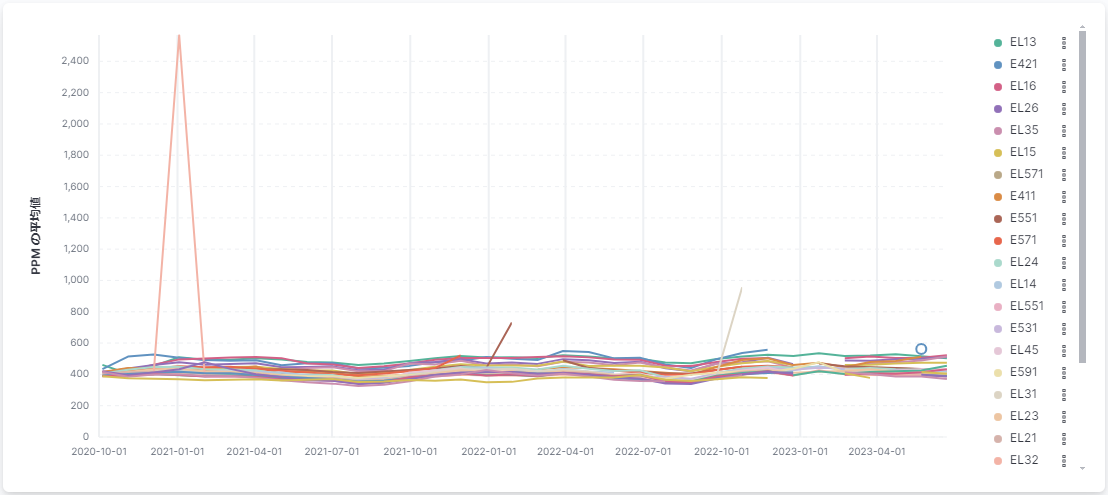
\includegraphics[width=170mm]{sotu/figure/ppm.png}
  \caption{co2\_modbusのPPM(30日間のPPMの平均値)}
  \label{p12}
\end{figure}

\begin{figure}[H]
  \hspace*{-2cm} % ここで左に2cmずらす
  \centering % center環境の代わりにこちらを使用
  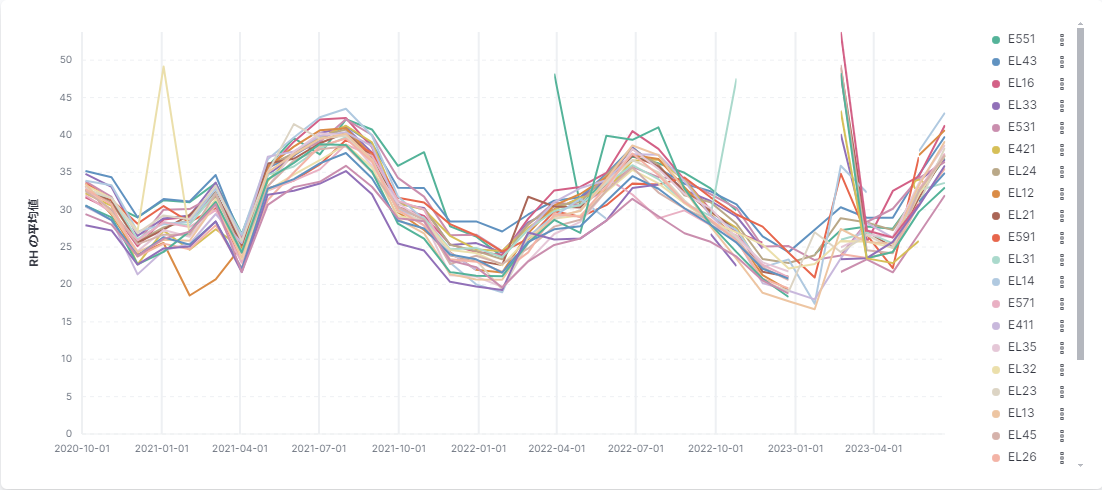
\includegraphics[width=170mm]{sotu/figure/rh.png}
  \caption{co2\_modbusのRH(30日間のRHの平均値)}
  \label{p13}
\end{figure}

\begin{figure}[H]
  \hspace*{-2cm} % ここで左に2cmずらす
  \centering % center環境の代わりにこちらを使用
  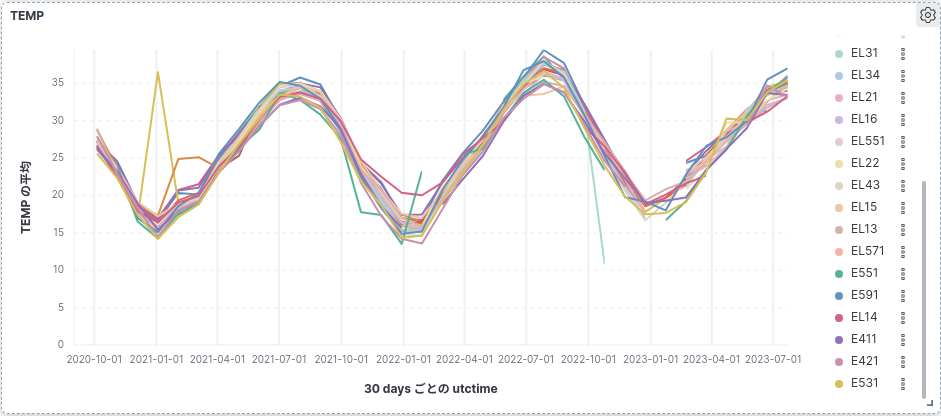
\includegraphics[width=170mm]{sotu/figure/temp.png}
  \caption{co2\_modbusの気温(30日間の気温の平均値)}
  \label{p14}
\end{figure}

図 \ref{p12} 〜 図 \ref{p14}より, 連続的にデータが変化していることが目視で確認できるので, データを欠落することなく重複データを削除出来たと判断した. なお, EL31教室にて気温が連続的に変化していないがこれはデータ計測システムが正常に動作せず計測出来ていなかったことが原因である. また, 2021年1月1日にE531教室の気温が他の教室より20℃程度高く計測されているが, これはセンサーの故障による誤った計測値であり, 連続的に変化しなくて良いデータである.

\section{LEAFの運行日誌に関するデータの移行手順について}

movement\_diary01インデックスのデータ移行は, 同名のインデックスを移行先のElasticSearchサーバーに作成して, 作成したインデックスにデータを挿入することで行う.

\subsection{データのエクスポート}
移行元のElasticSearchサーバーのデータのローカルマシンへのエクスポートには, elasticdumpライブラリを使用して, movement\_diary01インデックスの全ドキュメントをJSON形式でエクスポートした.

\subsection{データのインポート}
pythonのelasticsearchライブラリを使用し, 移行先のElasticsearchにmovement\_diary01という名前のインデックスを作成して, エクスポートしたデータを全てインサートした.

\section{KibanaによるLEAFの運行日誌に関するデータの可視化}

LEAFの運行日誌に関するデータを移行した後のmovement\_diary01インデックスについて, 横軸を計測時刻(dt\_S), 縦軸をbattery\_Sとしてプロットしたものを図 \ref{p15}に示す.

\begin{figure}[H]
  \hspace*{-2cm} % ここで左に2cmずらす
  \centering % center環境の代わりにこちらを使用
  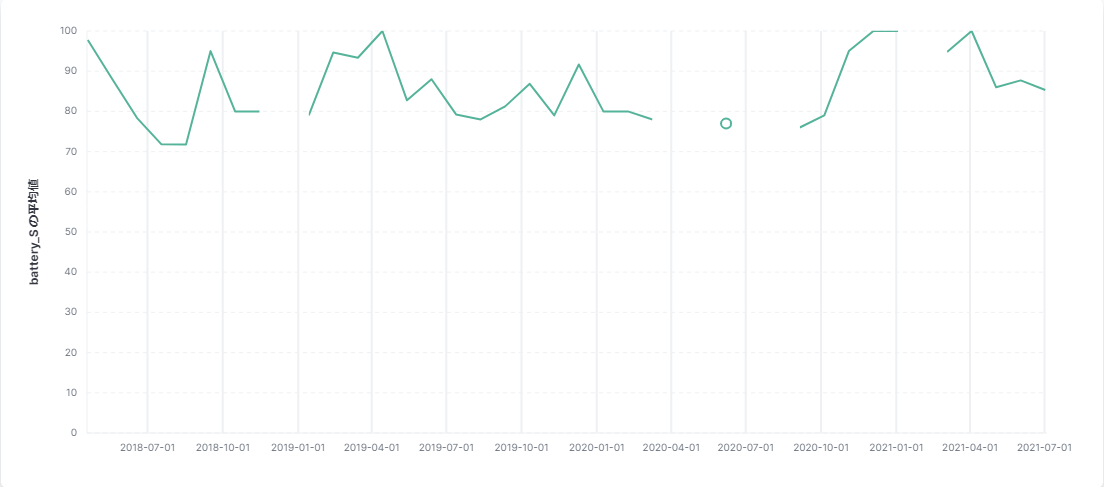
\includegraphics[width=170mm]{sotu/figure/battery-s.png}
  \caption{movement\_diary01のbattery\_S(30日間のbattery\_Sの平均値)}
  \label{p15}
\end{figure}

図 \ref{p15}より, 連続的にデータが変化していることが目視で確認できるので, データを移行出来たと判断した. なお, 連続的に変化していない箇所が複数存在するが, これはLEAFを稼働させていないことによるものであるため, 連続的に変化しなくて良いデータである.

\section{結言}
本章では単一ElasticsearchノードからElasticsearchクラスタへのデータ移行について述べた.

次章ではDockerによる仮想環境を使用したクラスタリング動作の可否の検証ついて述べる.   % 3章
\chapter{仮想環境を使用したクラスタリング動作の検証}
\label{chap:fourth}

\section{緒言}
本章ではDockerによる仮想環境を使用したクラスタリング動作の可否の検証ついて述べる.

% \section{サーバーゾーンで稼働しているElasticsearchシステムの状況}
% サーバーゾーンでは, 133.71.201.197で単一ノードのElasticsearchが稼働しており, リサイクル館の太陽光パネルの計測データが保存されている.

% 133.71.201.197のElasticsearchのバージョン7.17.6であり, 学内ゾーンで稼働しているElasticsearchクラスタに参加しているElastisearchノードのバージョンは7.17.9である.

% 本研究室では現在, バージョン7.17.9のElasticsearchを採用しているため, サーバーゾーンで構築しようとしているクラスタのElasticsearchのバージョンも, 学内ゾーンで稼働しているElasticsearchクラスタと同様, バージョン7.17.9を採用する.

% そこで, Docker, Docker Compose を使用して, 異なるバージョンである7.17.6 と 7.17.9 の Elasticsearch ノードをクラスタリングすることが可能かどうかを確認するために実施した.

\section{Dockerとは}
Dockerは, 軽量で独立したコンテナ型仮想環境用のプラットフォームである.

従来の仮想化では, VMWareなどの仮想化ソフトウェアを用いて, ホストOS上にゲストOSを構築する形式だった.
しかし, DockerはホストOS上にゲストOSなしで独立したコンテナ型の仮想環境として構築される.
Dockerコンテナを利用する場合は, Docker Engineをインストールすることでコンテナの立ち上げ, 停止, 削除といった操作を行うことができる.

\begin{figure}[H]
  \begin{center}
    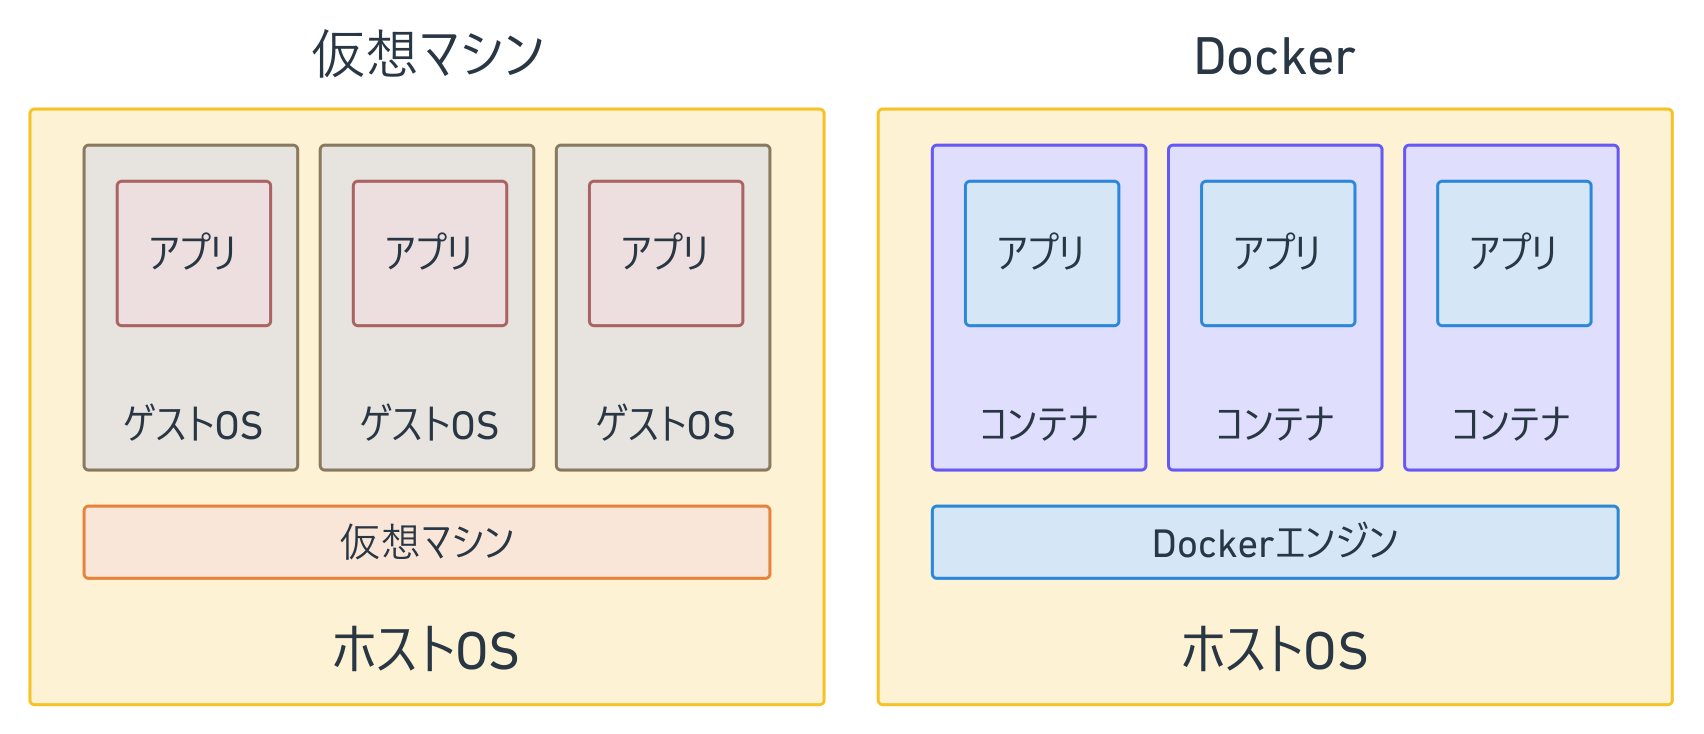
\includegraphics[width=120mm]{sotu/figure/docker-vmware.png}
    \caption{仮想マシンとDockerの違い \cite{3}}
    \label{4-p1}
  \end{center}
\end{figure}

\subsection{コンテナとは}

コンテナは, アプリケーションとそのすべての依存関係(ライブラリ, 実行環境など)をカプセル化した軽量な実行単位である.
Dockerの場合, コンテナの作成にはDockerイメージが必要となる.

\subsection{Dockerイメージとは}

Dockerイメージとは, Dockerコンテナを作成するためのテンプレートであり, Dockerイメージの中には, Docker コンテナの実行に必要な Linux ファイルシステムとメタ情報を含む.

Linux ファイルシステムというのは,  / ディレクトリ以下の /etc /bin /sbin /usr などのディレクトリ階層およびファイルである. 

Docker では, コンテナとして動かしたいアプリケーションが必要とする, 最小限のファイルを Docker イメージの中に入れる. 

さらに, そのアプリケーションを動かすために必要なデフォルトのコマンドや引数の指定, 外に公開するポート番号の情報などの情報がある. これらをメタ情報として, 同じく Docker イメージの中に入れられる 

DockerイメージはDocker Hubやその他のレジストリで共有されており, これらのサービスから取得することが可能である.

今回はElasticsearchの開発元であるElastic社が提供しているElasticsearchのDockerイメージを使って検証を行う.

\begin{figure}[H]
  \begin{center}
    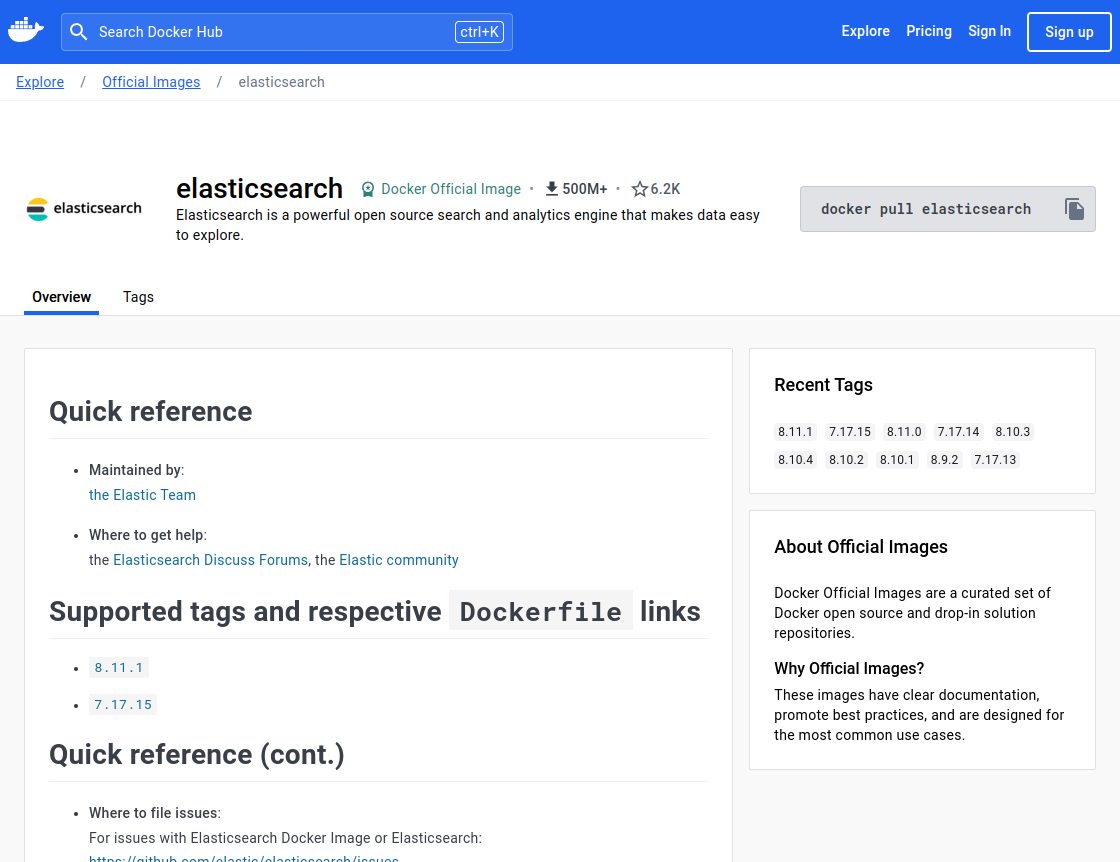
\includegraphics[width=120mm]{sotu/figure/elasticsearch-image.png}
    \caption{ElasticsearchのDockerイメージ}
    \label{4-p2}
  \end{center}
\end{figure}

\section{Docker Composeとは}
Docker Composeは, 複数のコンテナを定義し, 実行するためのツールである. これはYAMLファイルを使用して設定され, 複数のコンテナで協調して動作するアプリケーションの開発を単純化する.

\section{バージョンの異なるElasticsearchノードを用いたクラスタ構築の可否の検証}
\subsection{全て同じバージョンのElasticsearchを使用したクラスタ構成 (全ノード バージョン 7.17.9)}

% Listing \ref{sc1}に7.17.9バージョンのElasticsearchのみを使用してクラスタを構築した時のdocker-compose.ymlをを示す.

% \begin{lstlisting}[caption=全て同じバージョンのElasticsearchを使用したクラスタを構成するdocker-compose.yml, label=sc1]
%   version: '2.2'
%   services:
%     es01:
%       image: docker.elastic.co/elasticsearch/elasticsearch:7.17.9
%       container_name: es01
%       environment:
%         - node.name=es01
%         - cluster.name=es-docker-cluster
%         - discovery.seed_hosts=es02,es03
%         - cluster.initial_master_nodes=es01,es02,es03
%       ports:
%         - 9200:9200
%       networks:
%         - elastic
%     es02:
%       image: docker.elastic.co/elasticsearch/elasticsearch:7.17.9
%       container_name: es02
%       environment:
%         - node.name=es02
%         - cluster.name=es-docker-cluster
%         - discovery.seed_hosts=es01,es03
%         - cluster.initial_master_nodes=es01,es02,es03
%       networks:
%         - elastic
%     es03:
%       image: docker.elastic.co/elasticsearch/elasticsearch:7.17.9
%       container_name: es03
%       environment:
%         - node.name=es03
%         - cluster.name=es-docker-cluster
%         - discovery.seed_hosts=es01,es02
%         - cluster.initial_master_nodes=es01,es02,es03
%       networks:
%         - elastic

%   networks:
%     elastic:
%       driver: bridge
%   \end{lstlisting}

% また, 図 \ref{4-p3}にListing \ref{sc1}のdocker-compose.ymlを図で表現したものを示す.

図 \ref{4-p3}に, 7.17.9バージョンのElasticsearchのみを使用してクラスタを構築した時のdocker-compose.ymlを図で表現したものを示す.

\begin{figure}[H]
  \begin{center}
    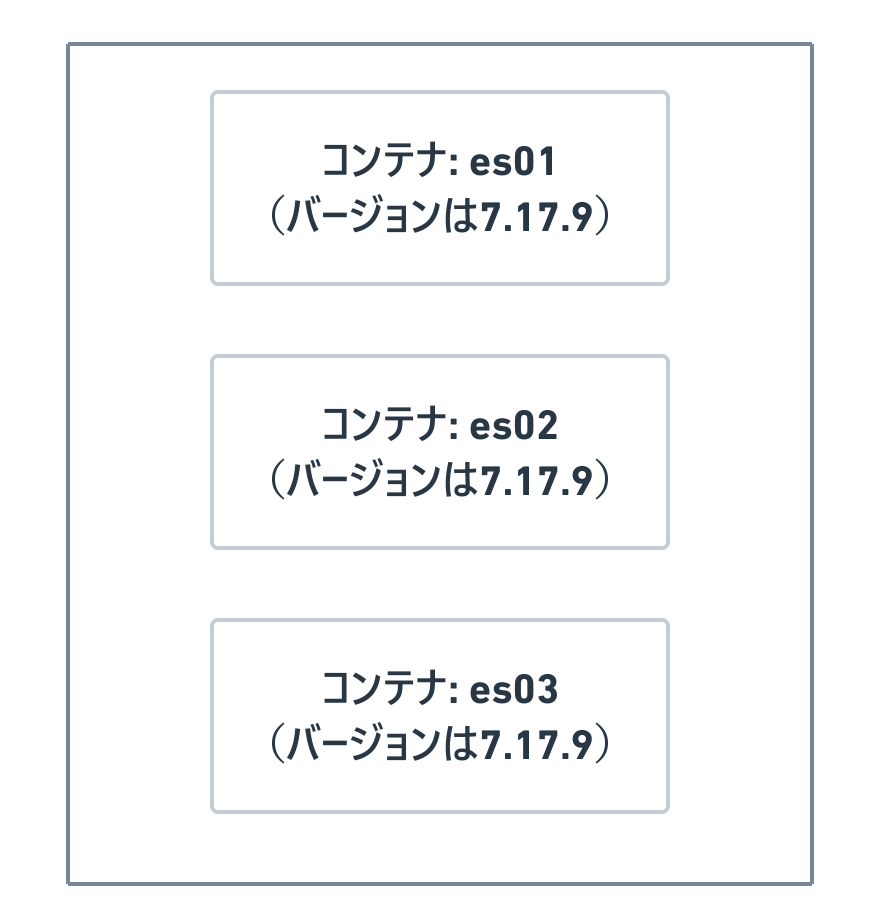
\includegraphics[width=120mm]{sotu/figure/all-7.19.9.png}
    \caption{docker-compose.ymlを図で表現したもの}
    \label{4-p3}
  \end{center}
\end{figure}

% Listing \ref{sc1}のdocker-compose.ymlファイルで記述している内容について説明する.

% \subsubsection*{サービスの定義}
% \begin{itemize}
%   \item \textbf{es01, es02, es03}: これらはElasticsearchのノード(サーバー)である. 各ノードは異なるコンテナとして定義されている. es01, es02, es03はそれぞれ異なるコンテナ名で, Elasticsearchの異なるインスタンスを実行する.
% \end{itemize}

% \subsubsection*{各ノードの設定}
% \begin{itemize}
%   \item \textbf{image}: 使用するDockerイメージ. ここではElasticsearchの7.17.9バージョンを使用している.
%   \item \textbf{container\_name}: コンテナに割り当てられる名前.
%   \item \textbf{environment}: 環境変数の設定. Elasticsearchのクラスタ設定を含む.
%   \item \textbf{ports}: ホストマシンとコンテナ間のポートマッピング. 例えば, `9200:9200`はホストマシンの9200ポートをコンテナの9200ポートにマッピングする.
%   \item \textbf{networks}: コンテナ間通信のためのネットワーク設定. ここではelasticネットワークが使用されている.
% \end{itemize}

% \subsubsection*{ボリュームとネットワークの設定}
% \begin{itemize}
%   \item \textbf{networks}: デフォルトのドライバであるbridgeドライバを使用するelasticネットワークを定義している. これにより, 異なるコンテナが相互に通信できるようになる.
% \end{itemize}

% この設定により, Elasticsearchの3ノードを含むクラスタがDocker上で動作するようセットアップされる.

% 以降, 説明を簡単にするため, docker-compose.ymlを図で表現したもののみを掲示する.

クラスタの起動には, docker compose up -dコマンドを使用する.

docker compose up -dコマンドを実行した後, curlコマンドを使用してクラスタに参加しているノードを一覧表示した結果を図 \ref{4-p4}に示す.

\begin{figure}[H]
  \begin{center}
    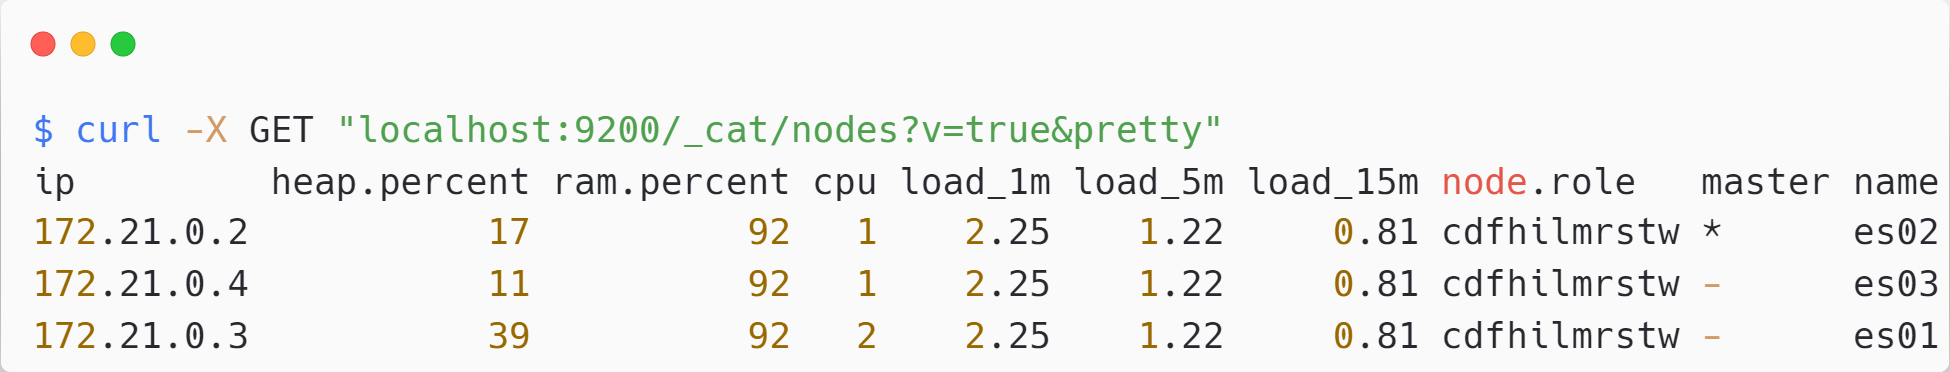
\includegraphics[width=140mm]{sotu/figure/curl-same.png}
    \caption{クラスタに参加しているノードを一覧表示した結果}
    \label{4-p4}
  \end{center}
\end{figure}

図 \ref{4-p4}より, 3つのノード(es01, es02, es03)すべてが正常にクラスタに参加できていることが確認できる.

\subsection{異なるバージョンのElasticsearchを使用したクラスタ構成 (2ノード バージョン 7.17.9, 1ノード バージョン 7.17.6)}

図 \ref{4-p3}で示されたdocker-compose.ymlにおいて, es03のコンテナで使用されるDockerイメージを変更して, Elasticsearchのバージョンを7.17.9から7.17.6にダウングレードする.

図 \ref{4-p5}に変更後のdocker-compose.ymlを図で表現したものを示す.

\begin{figure}[H]
  \begin{center}
    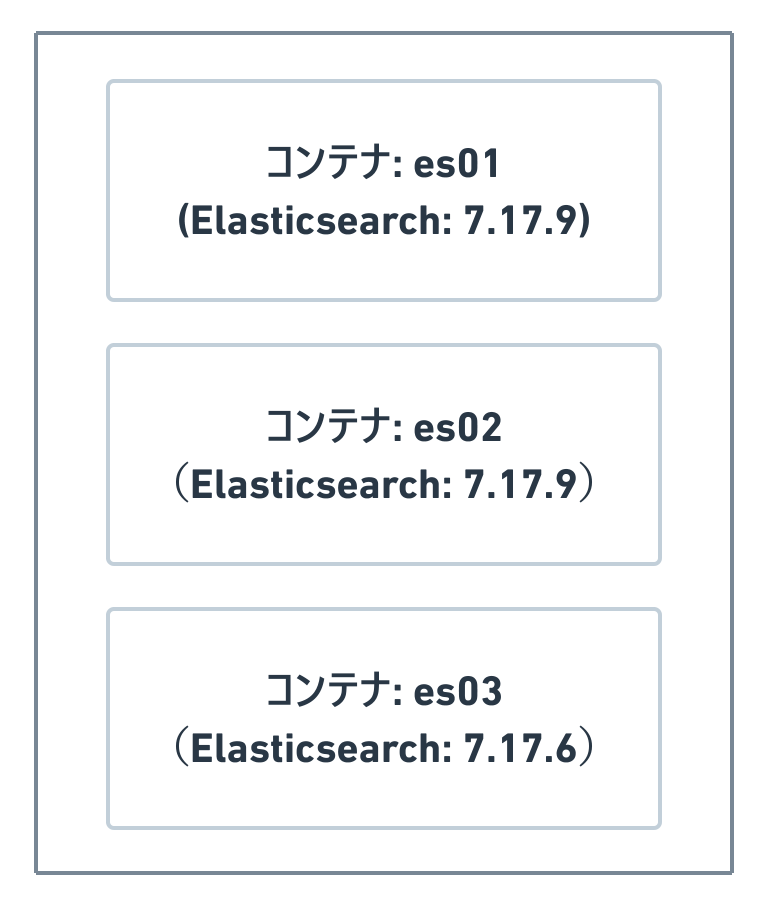
\includegraphics[width=120mm]{sotu/figure/2-7.19.9-and-1-7.17.6.png}
    \caption{変更後のdocker-compose.ymlを図で表現したもの}
    \label{4-p5}
  \end{center}
\end{figure}

変更後, docker compose up -dコマンドを実行してクラスタを起動する.

クラスタの起動後, curlコマンドを使用してクラスタに参加しているノードを一覧表示した結果を図 \ref{4-p6}に示す.

\begin{figure}[H]
  \begin{center}
    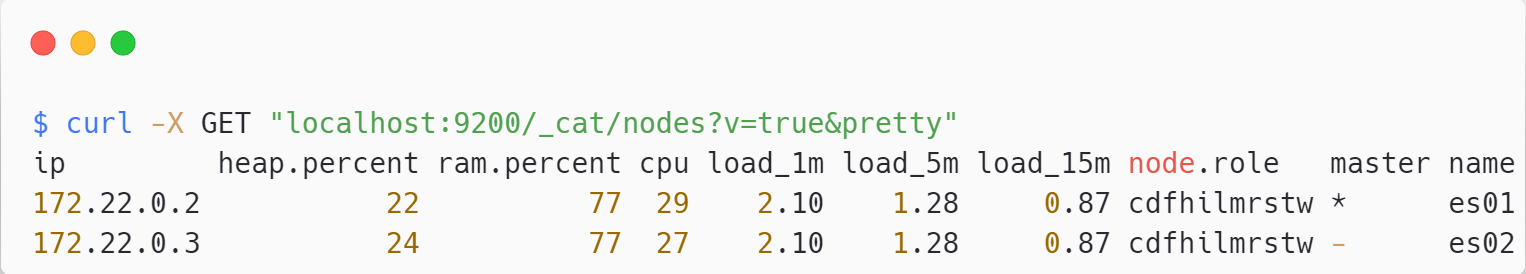
\includegraphics[width=140mm]{sotu/figure/curl-different.png}
    \caption{クラスタに参加しているノードを一覧表示した結果}
    \label{4-p6}
  \end{center}
\end{figure}

図 \ref{4-p6}より, Elasticsearchのバージョンが7.17.9である2つのノード(es01, es02)のみがクラスタに参加できていることが確認できる.

es03のコンテナでElasticsearchの起動を試みた時に出力されたログを確認したところ, 図 \ref{4-p7}に示すように, エラーログを出力して起動に失敗していた.

\begin{figure}[H]
  \begin{center}
    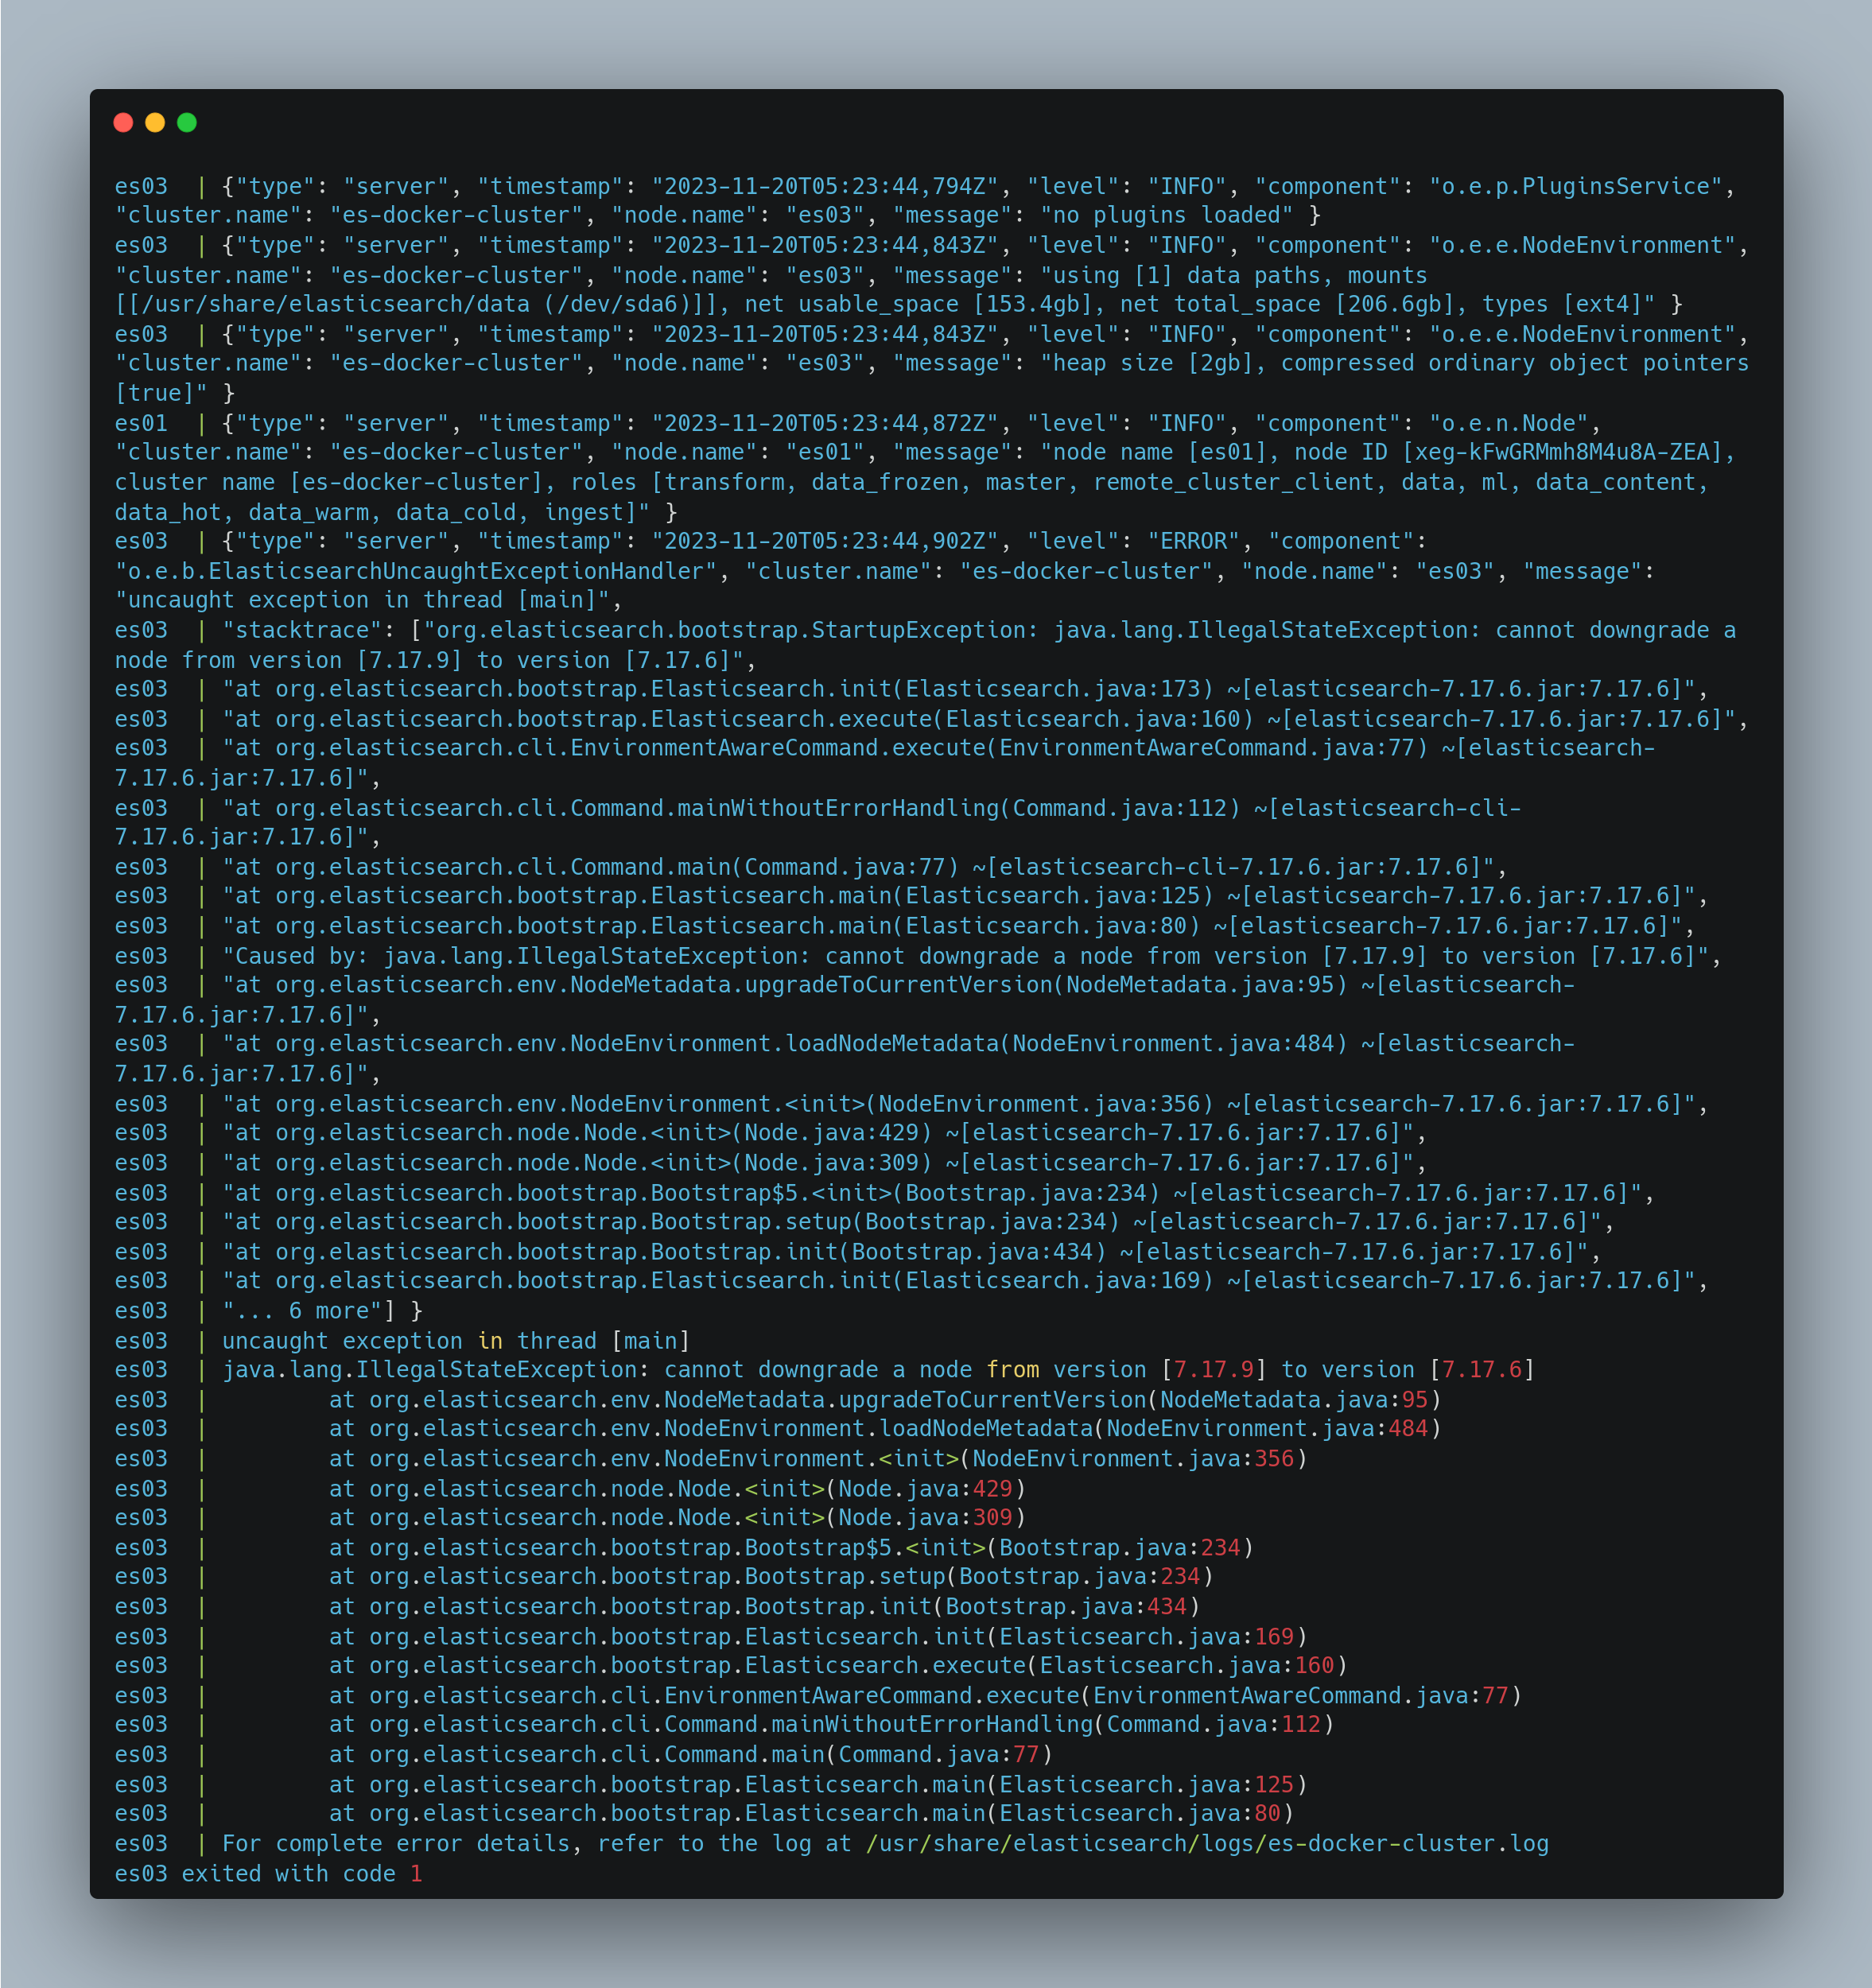
\includegraphics[width=140mm]{sotu/figure/log.png}
    \caption{es03のログ}
    \label{4-p7}
  \end{center}
\end{figure}

\section{既存Elasticsearchノードの異なるクラスタへの参加の可否の検証}
クラスタ構築において, 既に稼働しているElasticsearchノードを新たなノードとして異なるクラスタへ参加できるか, Dockerによる仮想環境を用いて検証した.

\subsection{単一ノードで稼働するクラスタAの構築}

まず, docker-composeを用いて単一ノード(コンテナ名はes04)でクラスタを構築する. 以後このクラスタをクラスタAと呼ぶ.

図 \ref{4-p8}にクラスタAを構築する際に使用したdocker-compose.ymlを図で表現したものを示す.

\begin{figure}[H]
  \begin{center}
    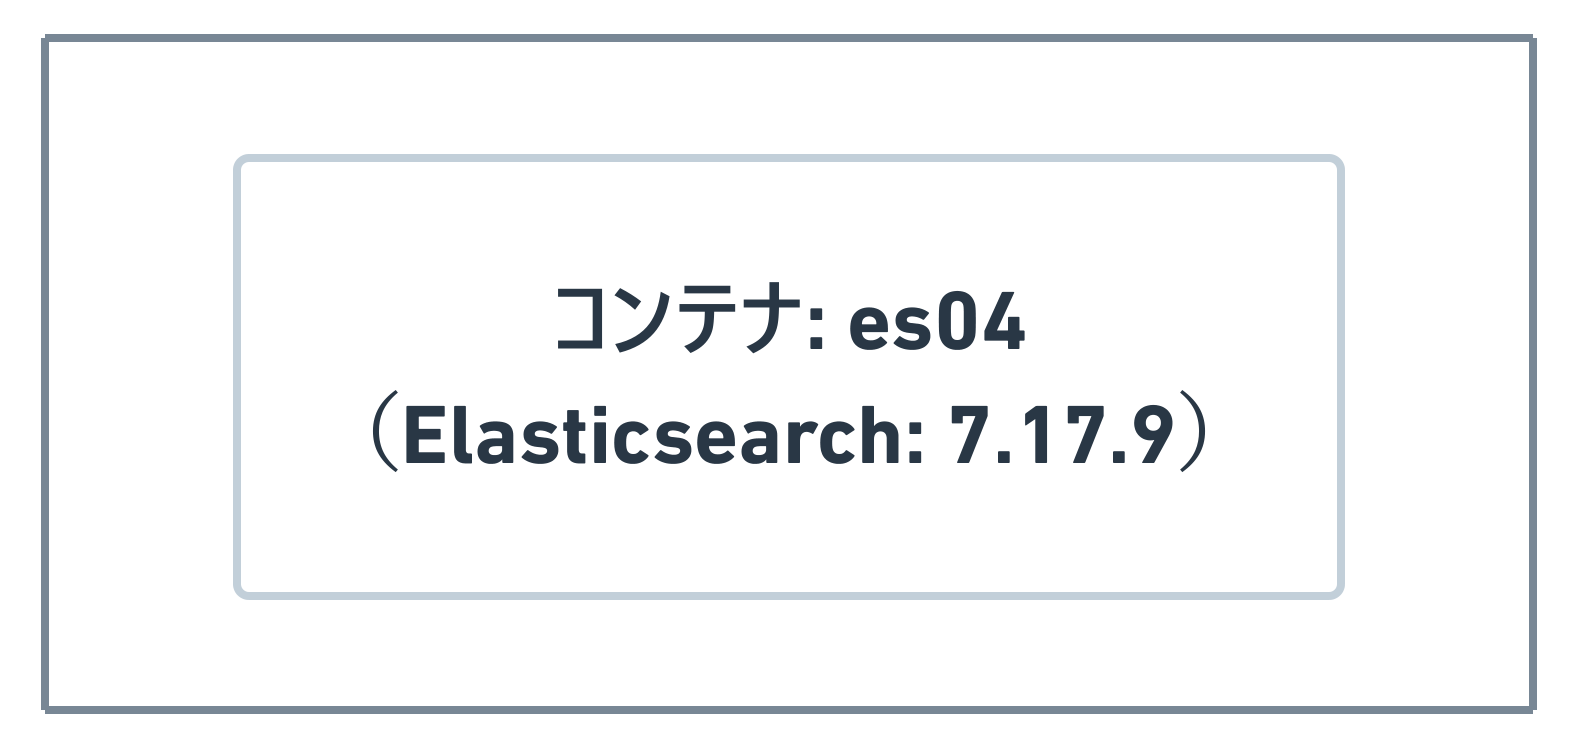
\includegraphics[width=100mm]{sotu/figure/1-7.17.9.png}
    \caption{クラスタAを構築する際に使用したdocker-compose.ymlを図で表現したもの}
    \label{4-p8}
  \end{center}
\end{figure}

docker-composeを用いてクラスタAを起動した後, クラスタの情報について問い合わせた結果を図 \ref{4-p9}に示す.

\begin{figure}[H]
  \begin{center}
    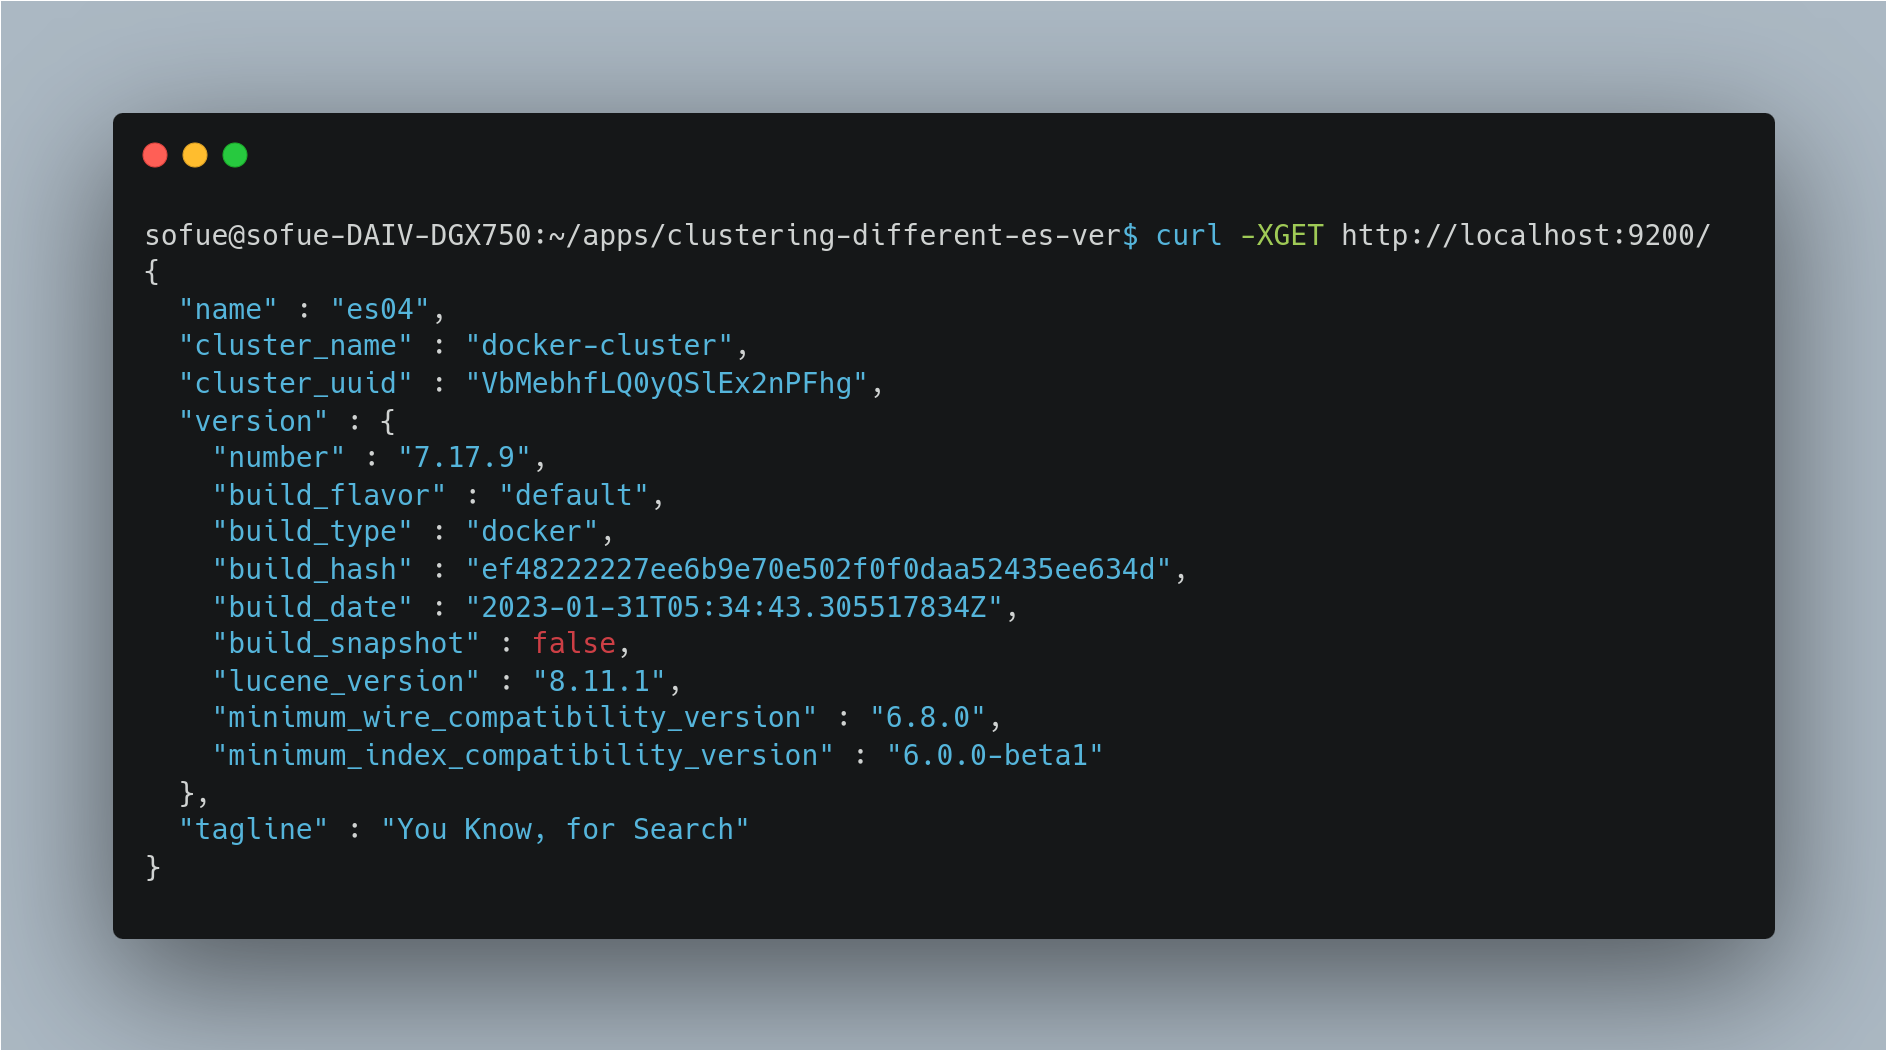
\includegraphics[width=140mm]{sotu/figure/es04-cluster.png}
    \caption{クラスタの情報について問い合わせた結果}
    \label{4-p9}
  \end{center}
\end{figure}

クラスタの情報について問い合わせた後, Dockerコンテナを停止してノードをシャットダウンした.

\subsection{3ノードで稼働するクラスタBの構築}

次に, クラスタAの構築に使用したノードとは別の3ノード(コンテナ名はそれぞれes01, es02, es03)でクラスタを構築する. 以後このクラスタをクラスタBと呼ぶ.

図 \ref{4-p10}にクラスタBの構築の際に使用したdocker-compose.ymlを図で表現したものを示す.

\begin{figure}[H]
  \begin{center}
    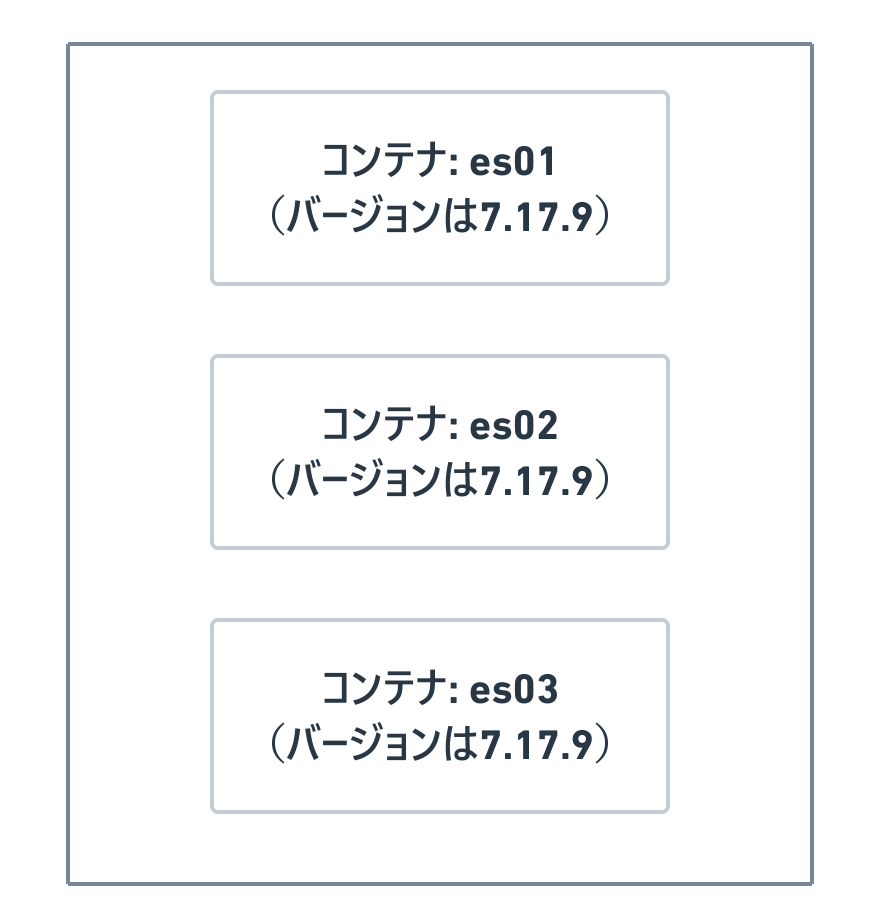
\includegraphics[width=120mm]{sotu/figure/all-7.19.9.png}
    \caption{クラスタBを構築する際に使用したdocker-compose.ymlを図で表現したもの}
    \label{4-p10}
  \end{center}
\end{figure}

docker-composeを用いてクラスタBを起動した後, クラスタの情報について問い合わせた結果を図 \ref{4-p11}に示す.

\begin{figure}[H]
  \begin{center}
    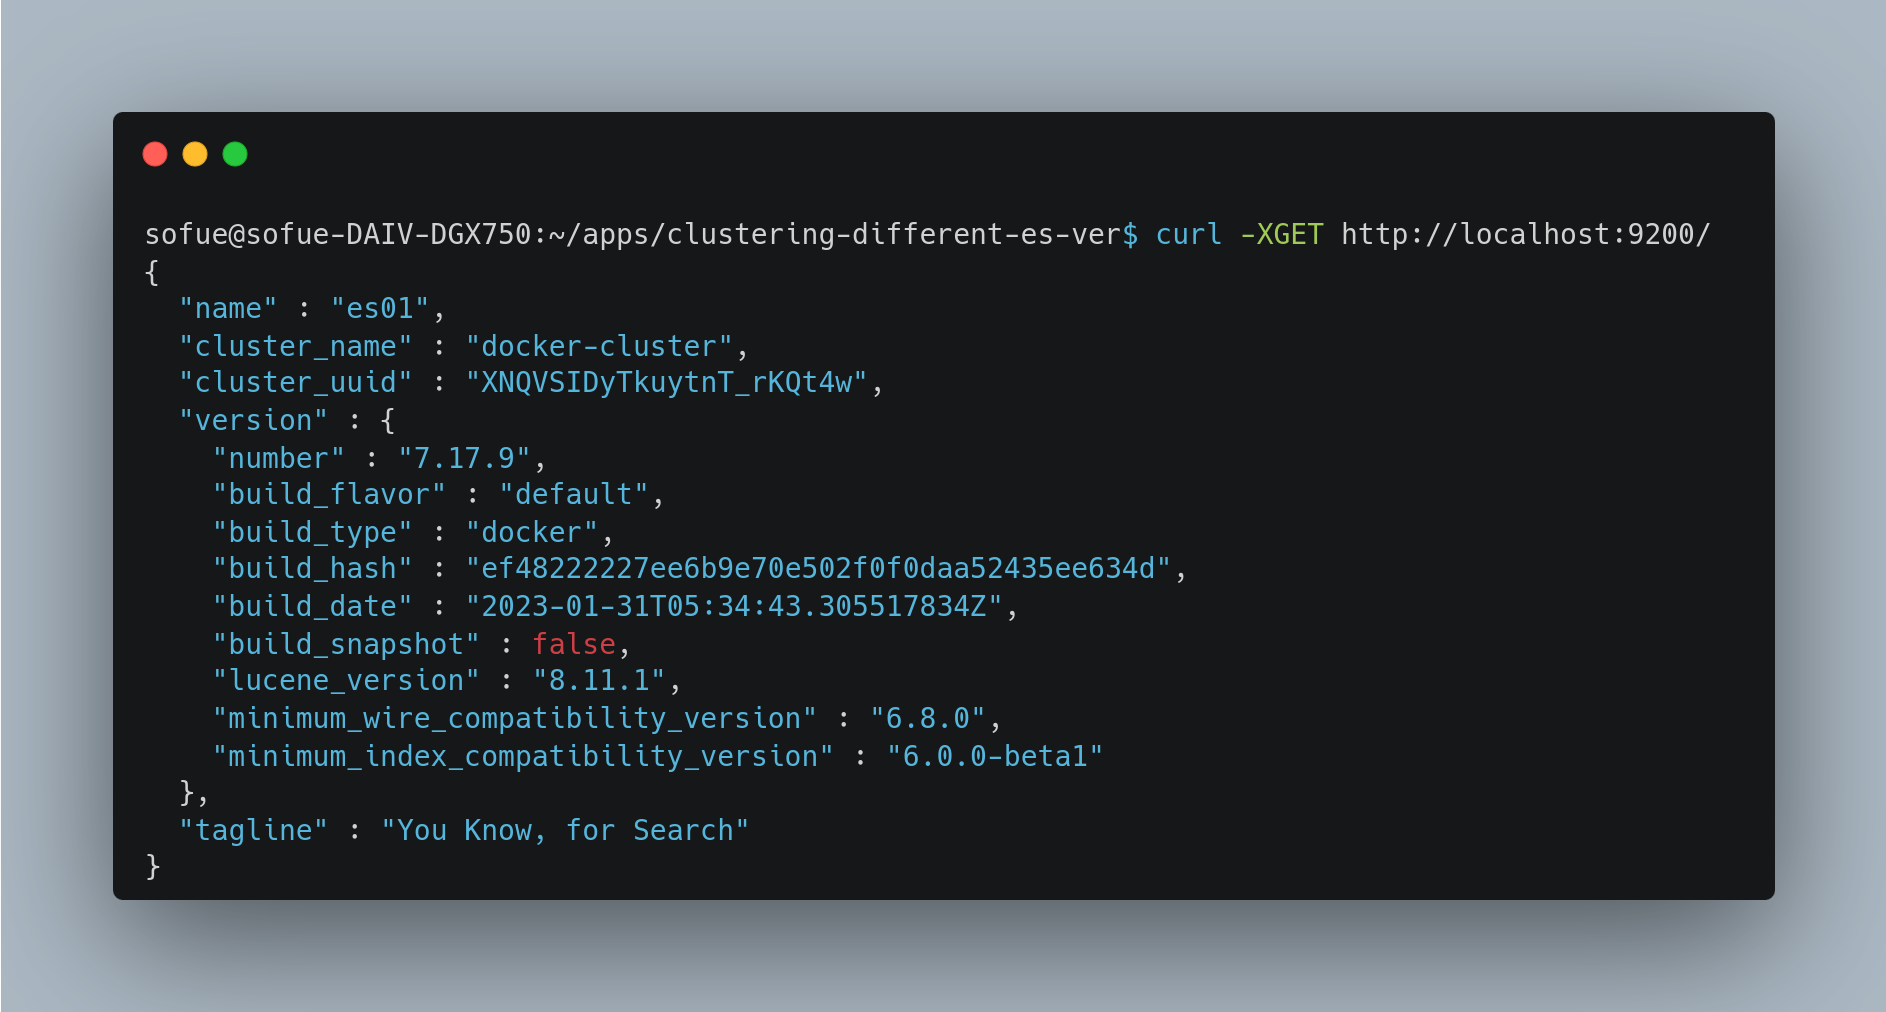
\includegraphics[width=140mm]{sotu/figure/3nodes-cluster.png}
    \caption{クラスタの情報について問い合わせた結果}
    \label{4-p11}
  \end{center}
\end{figure}

図 \ref{4-p9}と図\ref{4-p11}を比較した結果, クラスタAとクラスタBはそれぞれ異なるクラスタIDを付与されたことが分かった.

クラスタBの起動後, クラスタに参加しているノードの一覧を取得した結果を図 \ref{4-p12}に示す.

\begin{figure}[H]
  \begin{center}
    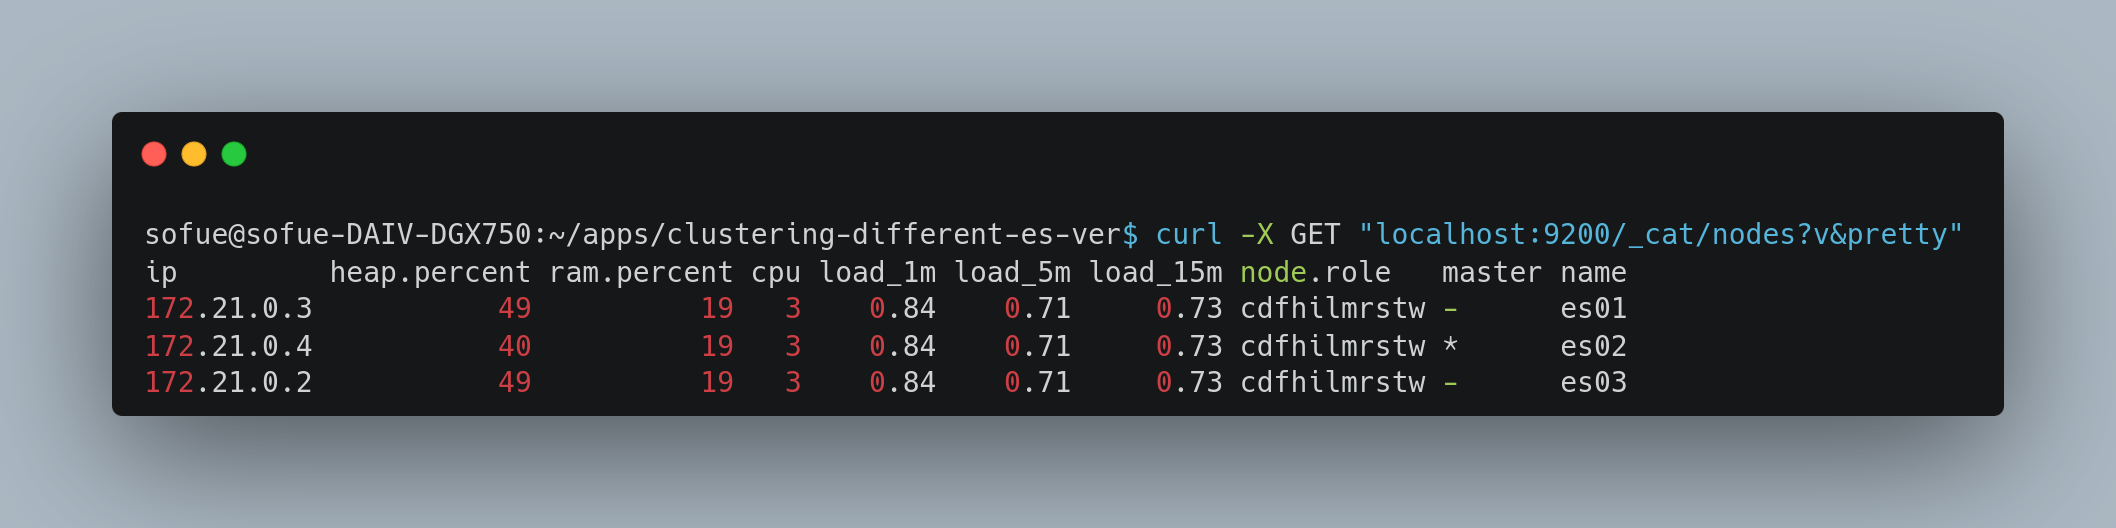
\includegraphics[width=140mm]{sotu/figure/3nodes-list.png}
    \caption{クラスタBの起動後, クラスタに参加しているノードの一覧を取得した結果}
    \label{4-p12}
  \end{center}
\end{figure}

図 \ref{4-p12}より, es01, es02, es03ノードがクラスタBに参加できていることを確認した.

クラスタBに参加しているノードの一覧を取得した後, 全てのDockerコンテナを停止してノードを全てシャットダウンした.

\subsection{クラスタAに参加しているノードのクラスタBへの参加試行}

次に, 図 \ref{4-p10}のdocker-compose.ymlに対して, クラスタAのノード(es04コンテナ)を追加し, 合計4ノードでのクラスタBの起動を試みる.

図 \ref{4-p13}に, es04コンテナを含めた4ノードでクラスタBの起動を試みた際に使用したdocker-compose.ymlを図で表現したものを示す.

\begin{figure}[H]
  \begin{center}
    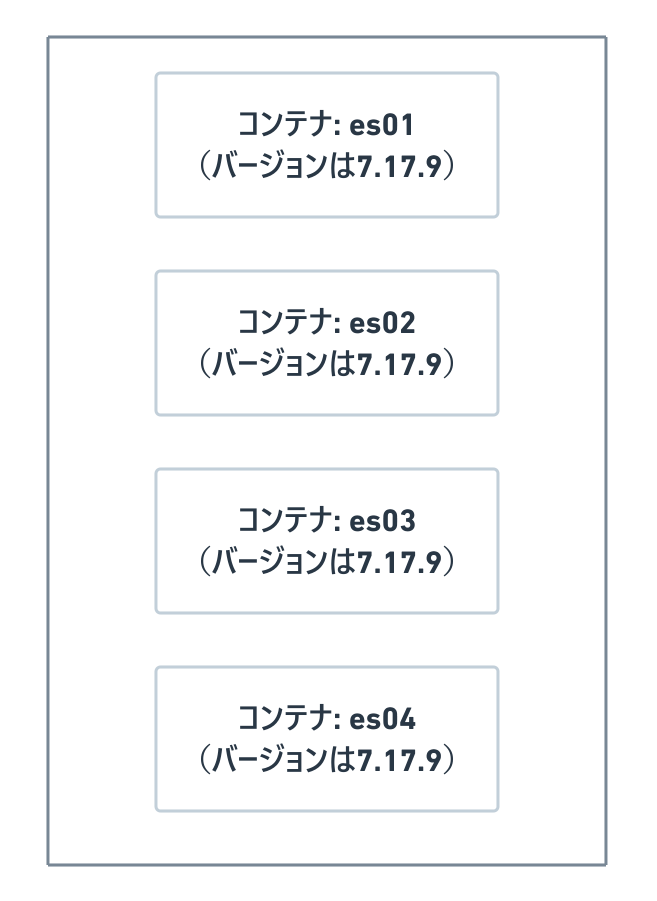
\includegraphics[width=120mm]{sotu/figure/4-7.17.9.png}
    \caption{es04コンテナを含めた4ノードでクラスタBの起動を試みた際に使用したdocker-compose.ymlを図で表現したもの}
    \label{4-p13}
  \end{center}
\end{figure}

クラスタBの起動後, クラスタに参加しているノードの一覧を取得した結果を図 \ref{4-p14}に示す.

\begin{figure}[H]
  \begin{center}
    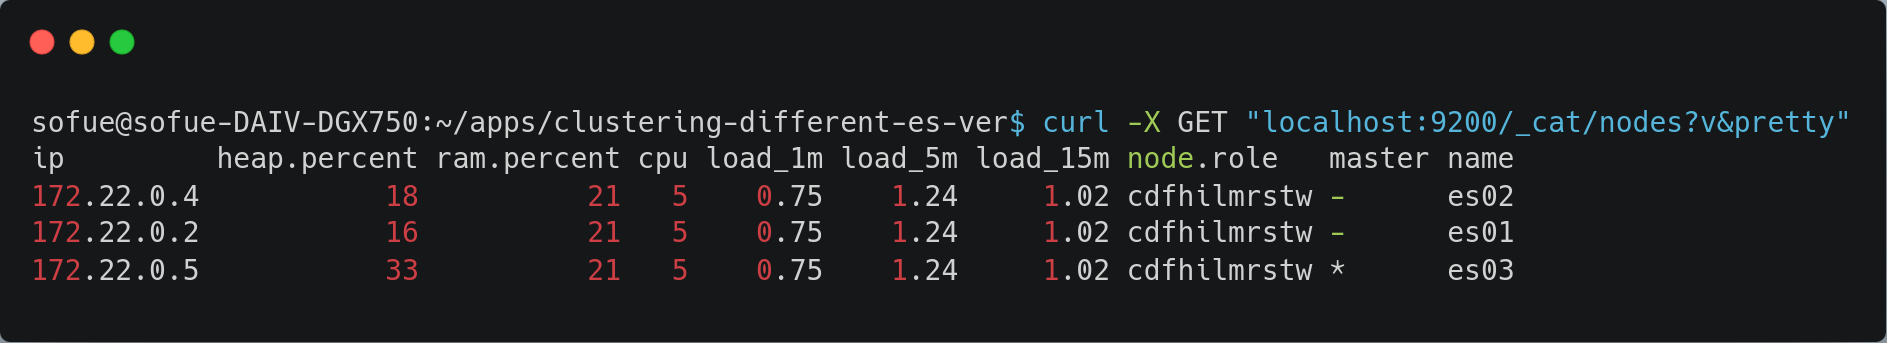
\includegraphics[width=140mm]{sotu/figure/4nodes-list.png}
    \caption{es04コンテナを含めたノードでクラスタBの起動を試みた後, クラスタに参加しているノードの一覧を取得した結果}
    \label{4-p14}
  \end{center}
\end{figure}

図 \ref{4-p14}より, クラスタAのノードがクラスタBに参加できていないことを確認した.

es04コンテナ(クラスタAに参加しているノード)で出力されたログの一部を図 \ref{4-p15}に示す.

\begin{figure}[H]
  \begin{center}
    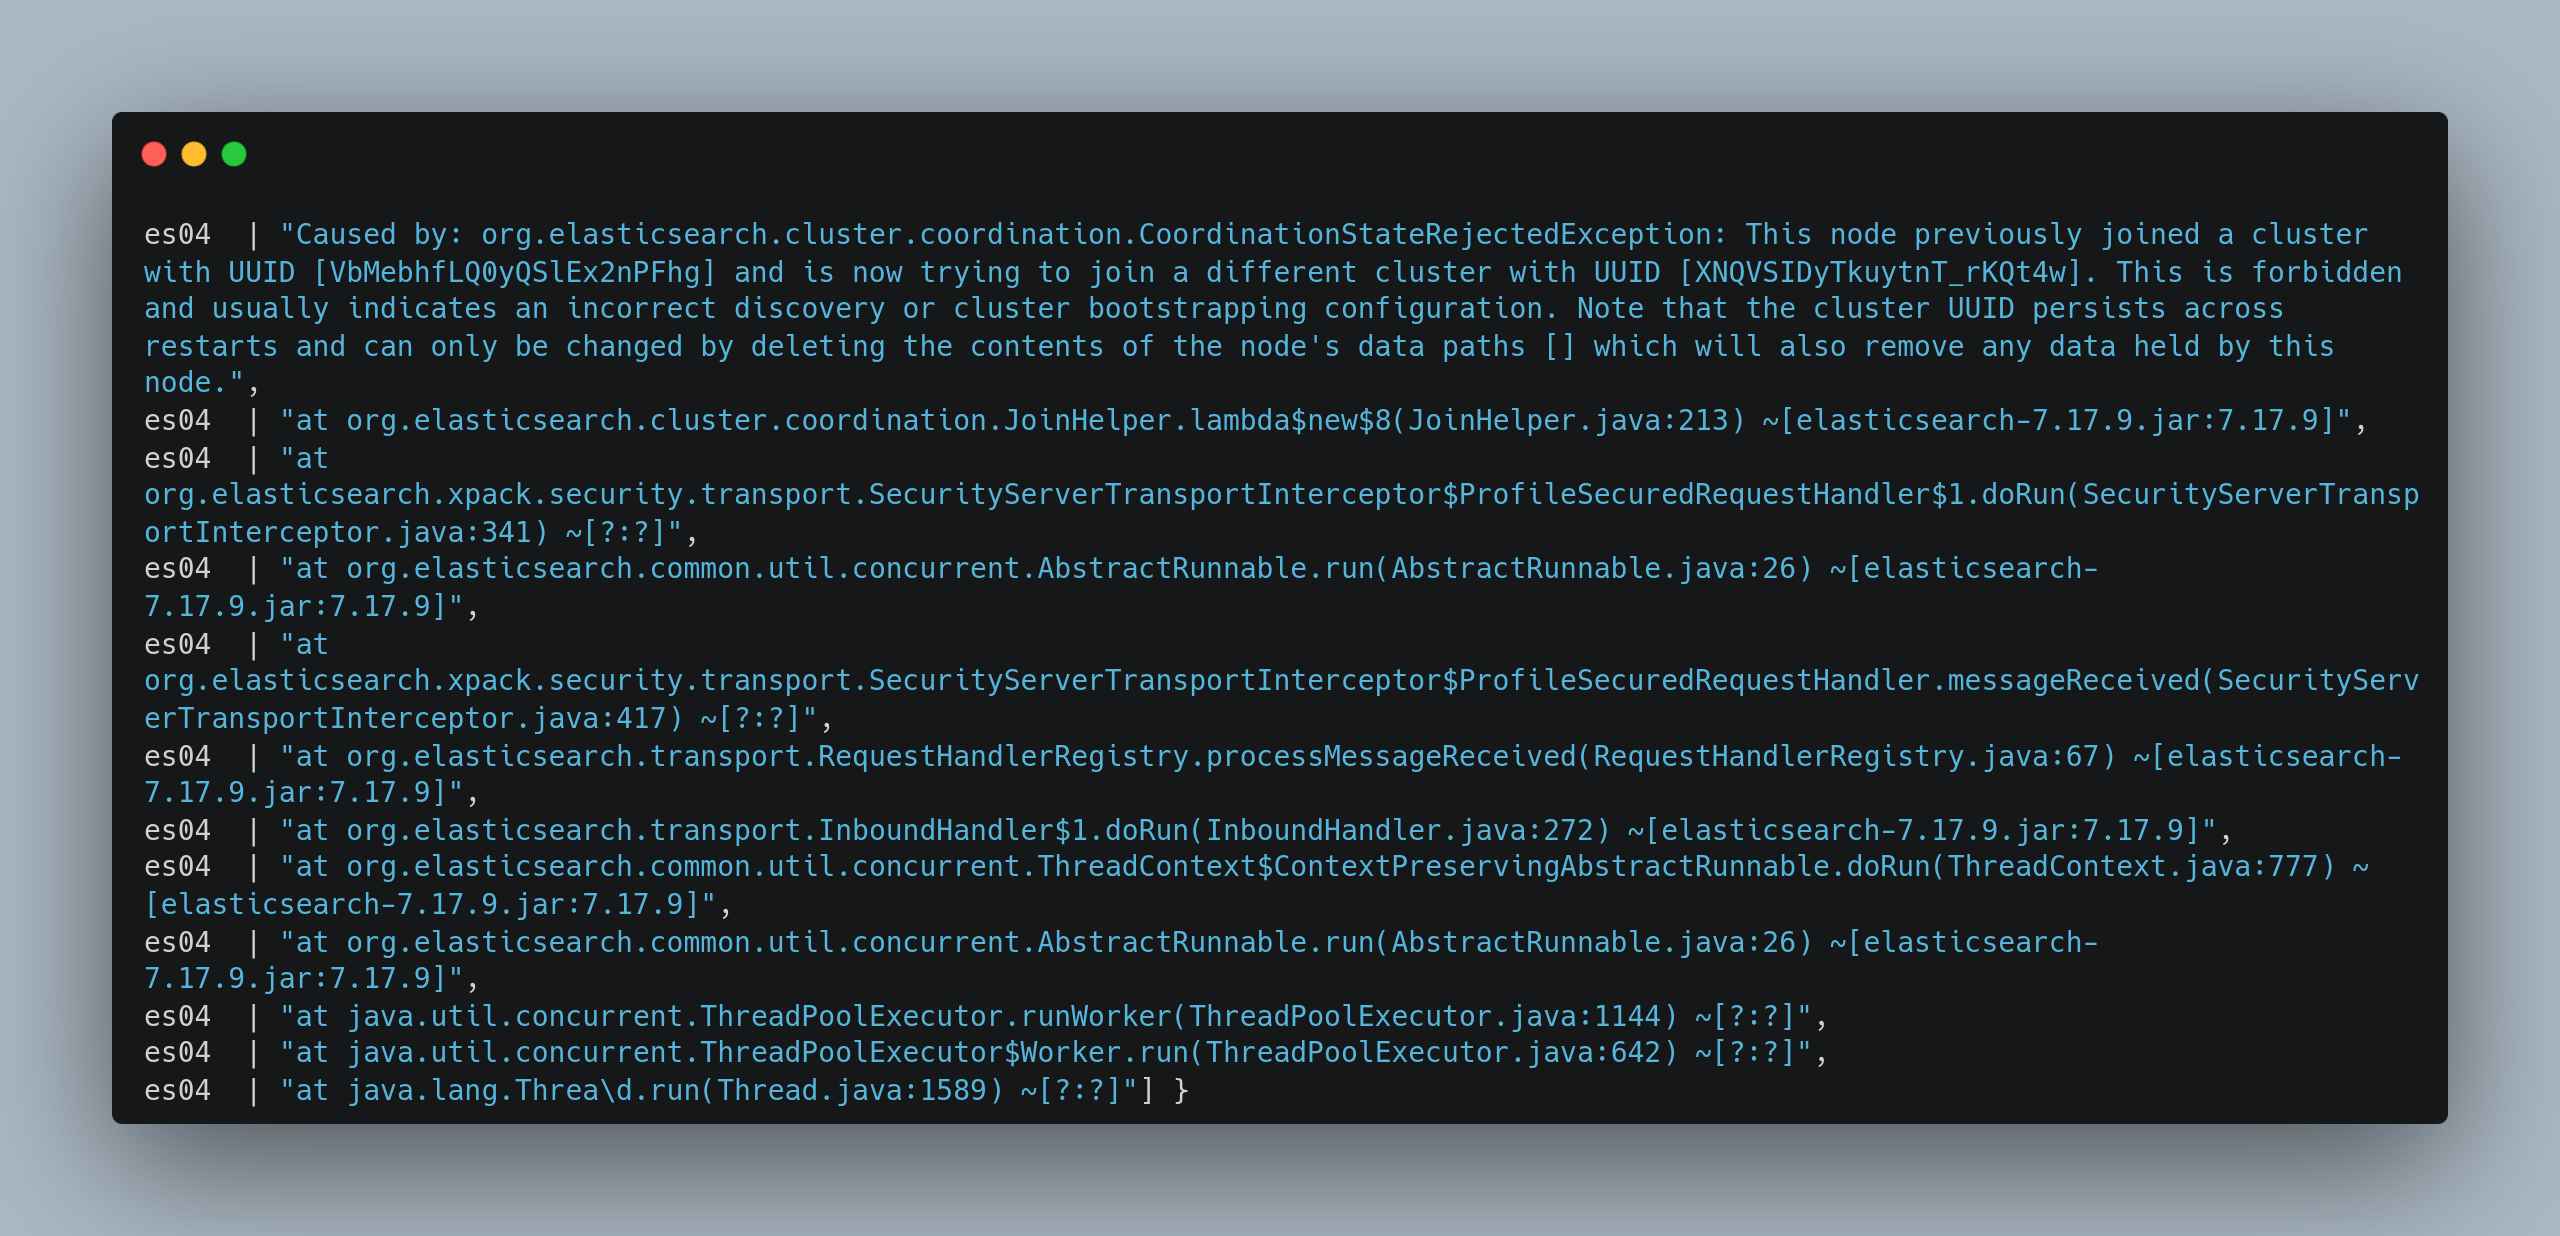
\includegraphics[width=140mm]{sotu/figure/es04-log.png}
    \caption{es04コンテナのログの一部}
    \label{4-p15}
  \end{center}
\end{figure}

図 \ref{4-p15}では, 異なるクラスタIDを持つクラスタにノードが参加することは禁止されており, 参加するためにはインデックスやドキュメント情報などが格納されているデータパス配下のフォルダ, ファイルを削除する必要があると書かれている.

以上の検証結果から, 既に稼働しているノードを別のクラスタに新しいノードとして参加させることは出来ないことが分かった.

% したがって, リサイクル館の太陽光パネルの計測データが保存されたElasticsearchノードをクラスタに参加させるには以下の2通りの方法が考えられる.

% \begin{itemize}
%   \item リサイクル館の太陽光パネルの計測データが保存されたElasticsearchノードのバックアップを取り, ノードに保存されたインデックスやドキュメントのデータを削除した上で, CO\textsubscript{2}データなどが保存されたクラスタに新しいノードとして参加させる
%   \item CO\textsubscript{2}データなどが保存されたクラスタとは別で, サーバーゾーンに新たにクラスタを構築する. クラスタの構築にはリサイクル館の太陽光パネルの計測データが保存されたElasticsearchノードが所属するクラスタを使用する.
% \end{itemize}

% 本来であれば、次の章の内容

% \section{Elasticsearchのバージョンアップ}
% 3章の検証結果より, 異なるバージョンのElasticsearchノードでクラスタを構築することは出来ないため, リサイクル館の太陽光パネルの計測データを保存しているElasticsearch(133.71.201.197)をバージョンアップする必要がある. そこで, 133.71.201.197にインストールされたElasticsearchのバージョンアップを行う.

% \section{バージョンアップ手順}

% \subsection{インストール方法の特定}

% バージョンアップを行うためには, 133.71.201.197のUbuntuPCにどのようにElasticsearchをインストールしたか特定する必要がある.

% 図 \ref{4-p16}に, aptによってインストールされたパッケージの中にelasticsearchという文字列を含むパッケージが存在するか調べた結果を示す.
% 図 \ref{4-p16}より, aptによってインストールされたことが分かった.

% \begin{figure}[H]
%   \begin{center}
%     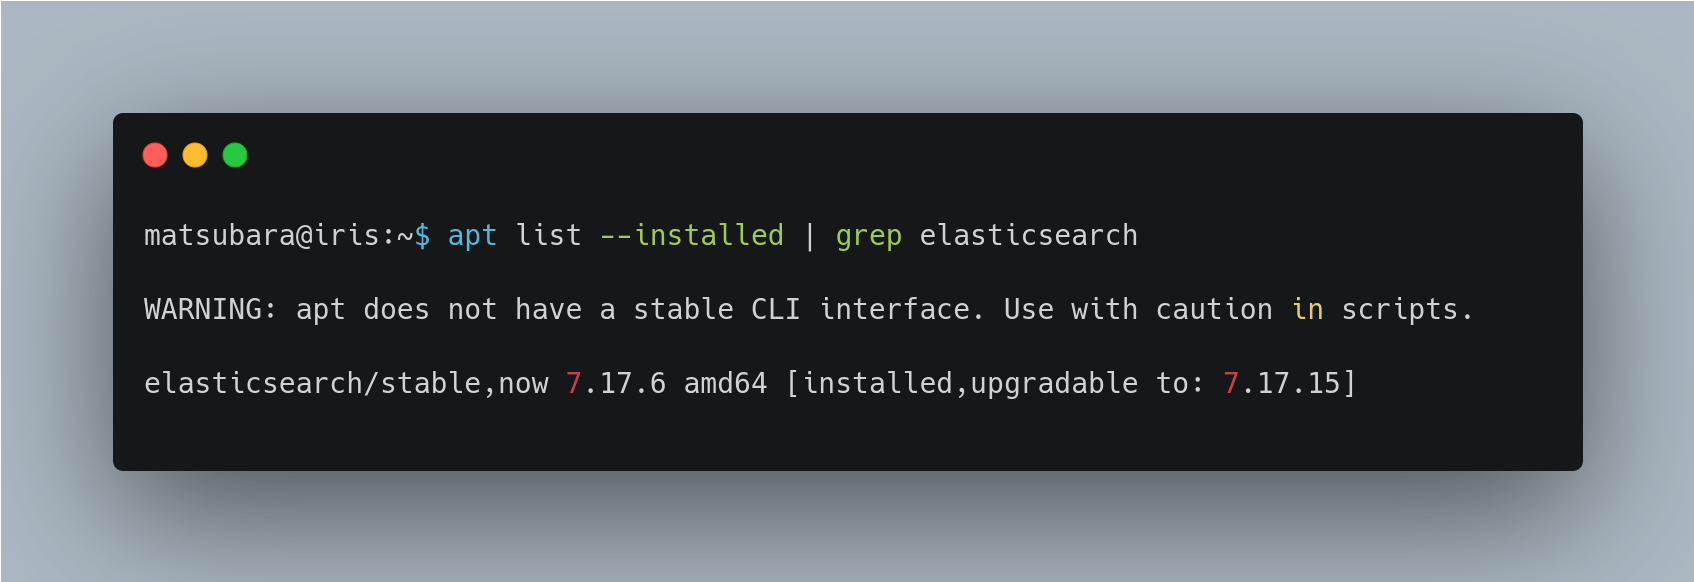
\includegraphics[width=120mm]{sotu/figure/apt-grep.png}
%     \caption{aptによってelasticsearchがインストールされたか調べた結果}
%     \label{4-p16}
%   \end{center}
% \end{figure}

% 次に, aptでインストール可能なelasticsearchのバージョンを一覧表示した結果を図 \ref{4-p17}に示す. 図 \ref{4-p17}にターゲットである7.17.9が含まれているため, aptを使用してバージョンアップできることが確認できた.

% \begin{figure}[H]
%   \begin{center}
%     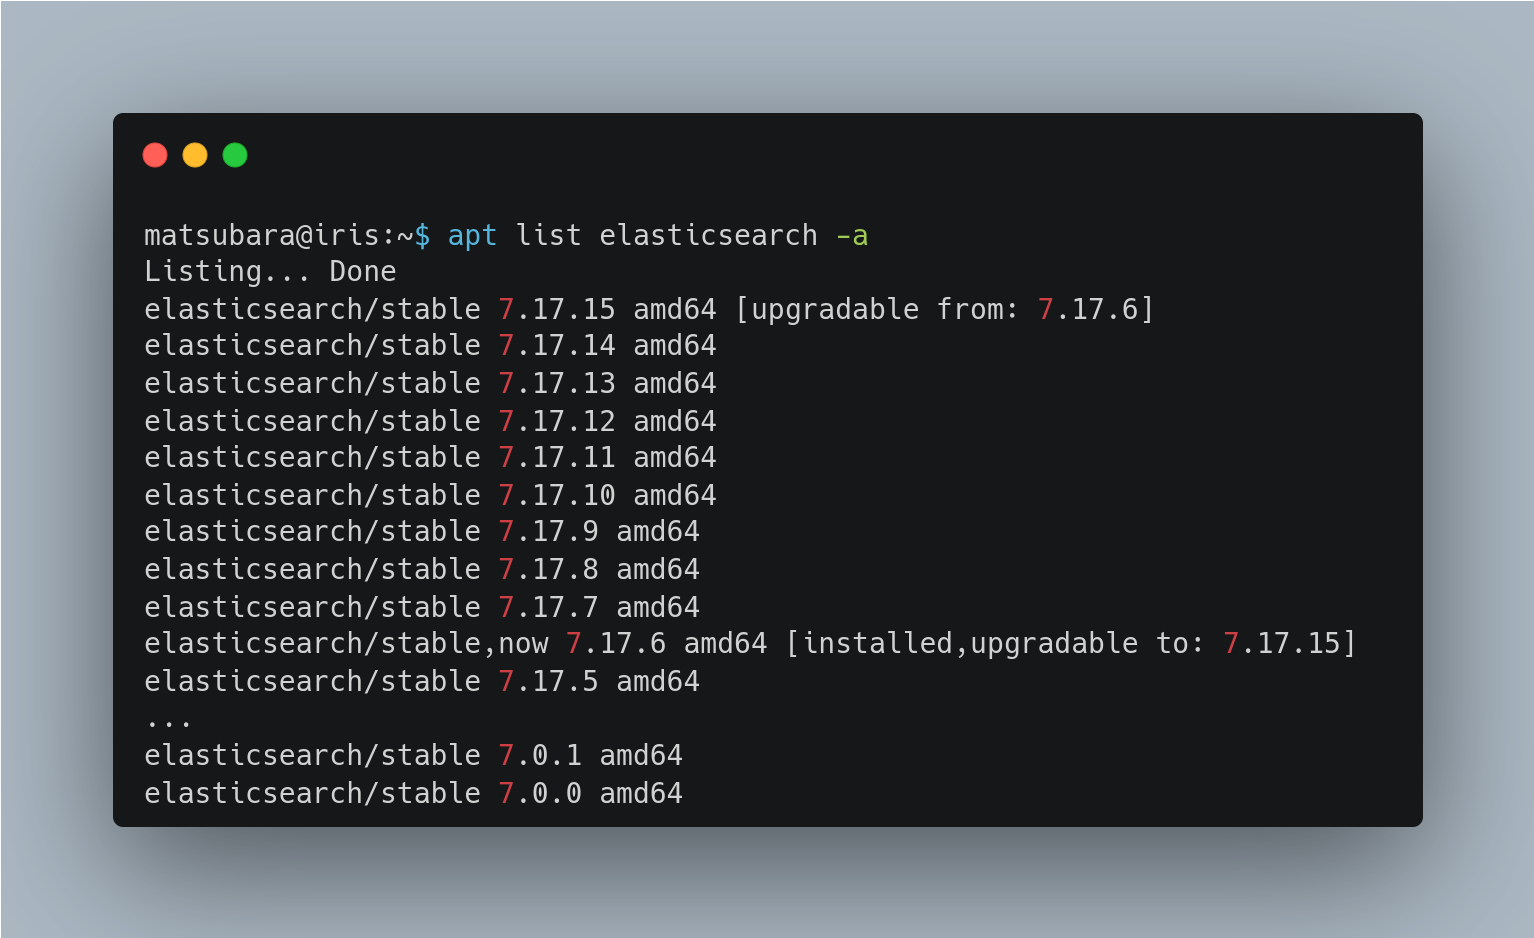
\includegraphics[width=120mm]{sotu/figure/apt-list.png}
%     \caption{aptでインストール可能なelasticsearchのバージョンを一覧表示した結果}
%     \label{4-p17}
%   \end{center}
% \end{figure}

% \subsection{aptによるバージョンアップ}

% まず, \textbf{sudo systemctl stop elasticsearch.service}コマンドを実行してelasticsearchノードをシャットダウンする.

% 次に, \textbf{sudo apt install elasticsearch=7.17.9}コマンドを実行してelasticsearchパッケージをバージョンアップする.

% elasticsearchをバージョンアップ後, \textbf{sudo systemctl start elasticsearch}コマンドを実行してElasticsearchノードを起動する.

% ノードの起動後, Elasticsearchのバージョンを確認した結果を図 \ref{4-p18}に示す.

% \begin{figure}[H]
%   \begin{center}
%     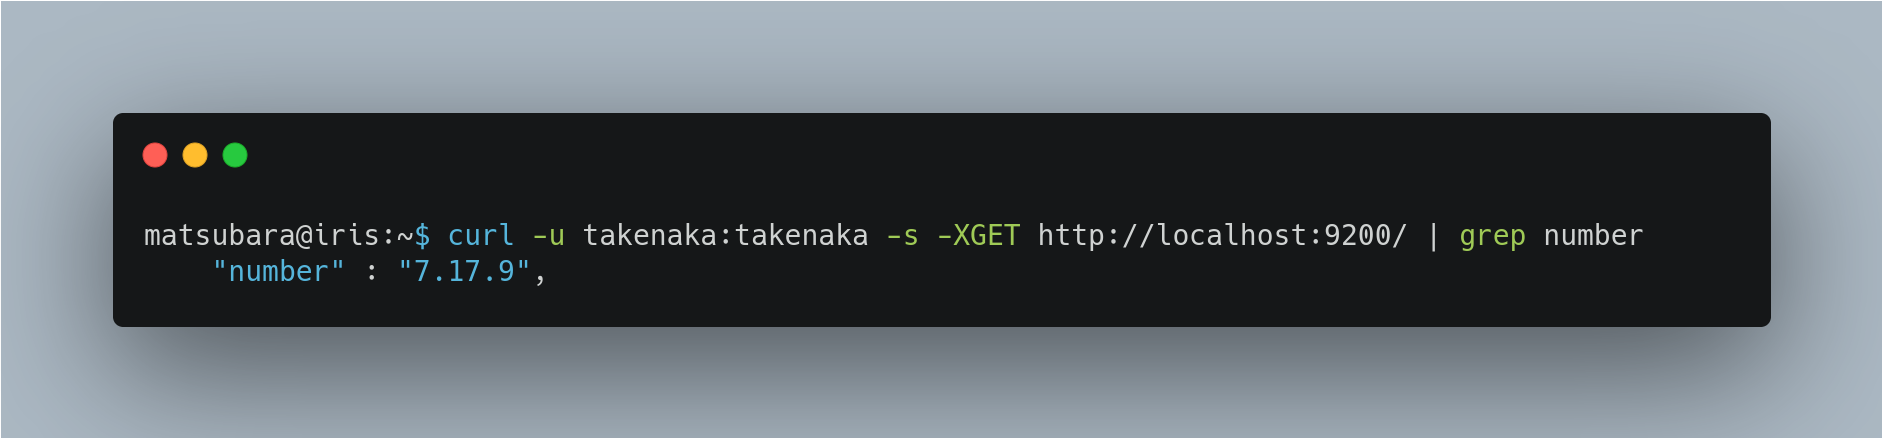
\includegraphics[width=140mm]{sotu/figure/version-check.png}
%     \caption{ノードの起動後, Elasticsearchのバージョンを確認した結果}
%     \label{4-p18}
%   \end{center}
% \end{figure}

% 図 \ref{4-p18}より, Elasticsearchのバージョンが7.17.9にバージョンアップ出来たことが確認できた.

% \section{Kibanaのバージョンアップ}

% Kibanaもelasticsearchと同様, aptを使用してインストールされていたため, \textbf{sudo systemctl stop Kibana.service}コマンド, \textbf{sudo apt install Kibana=7.17.9}コマンド, \textbf{sudo systemctl start Kibana}コマンドをそれぞれ実行して, Kibanaのバージョンアップも行った.

% \section{バージョンアップ後の動作確認}

% Elasticsearchのバージョンアップ後, 太陽光パネルの計測データがElasticsearchに保存されているかKibana上で確認した結果を図 \ref{p4}に示す.

% \begin{figure}[H]
%   \begin{center}
%     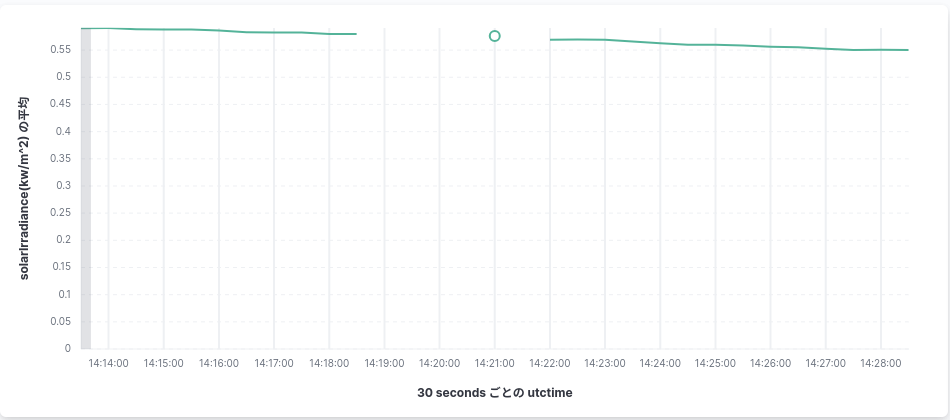
\includegraphics[width=140mm]{sotu/figure/downtime.png}
%     \caption{Elasticsearchのバージョンアップ後, 太陽光パネルの計測データが保存されているかKibana上で確認した結果}
%     \label{4-p19}
%   \end{center}
% \end{figure}

% 図 \ref{4-p19}より, バージョンアップ後のElasicsearchノードを起動した14:22:00以降にドキュメントがインサートされていることが確認できた.

\section{結言}
% 本章ではDockerによる仮想環境を使用したクラスタリング動作の可否の検証ついて述べた.

本章では, 異なるバージョンのElasticsearchノードを用いたクラスタリングの動作の検証と, 異なるクラスタへの Elasticsearchノードの参加の可否の検証を行った.

はじめに, 異なるバージョンのElasticsearchノードのクラスタリングを検証した. まず同じバージョンのElasticsearchノードを用いてクラスタを構築した後, 異なるバージョンの Elasticsearchノードを新たにクラスタに含めてクラスタ起動を試みたが, バージョンの不一致によりクラスタリングは失敗した. これにより, 異なるバージョンのElasticsearchノードを用いたクラスタ構築は出来ないことを確認した.

次に, 既に稼働している Elasticsearchノードを異なるクラスタに参加させる検証を行った. まずクラスタAとクラスタBをそれぞれ構築した後, クラスタAの ElasticsearchノードをクラスタBの Elasticsearchノードとして参加させて, クラスタBの起動を試みた. しかし, クラスタAの ElasticsearchノードはクラスタBに参加できなかった. これにより, 既に稼働している Elasticsearchノードを異なるクラスタに参加させることは出来ないことを確認した.

\begin{figure}[H]
  \begin{center}
    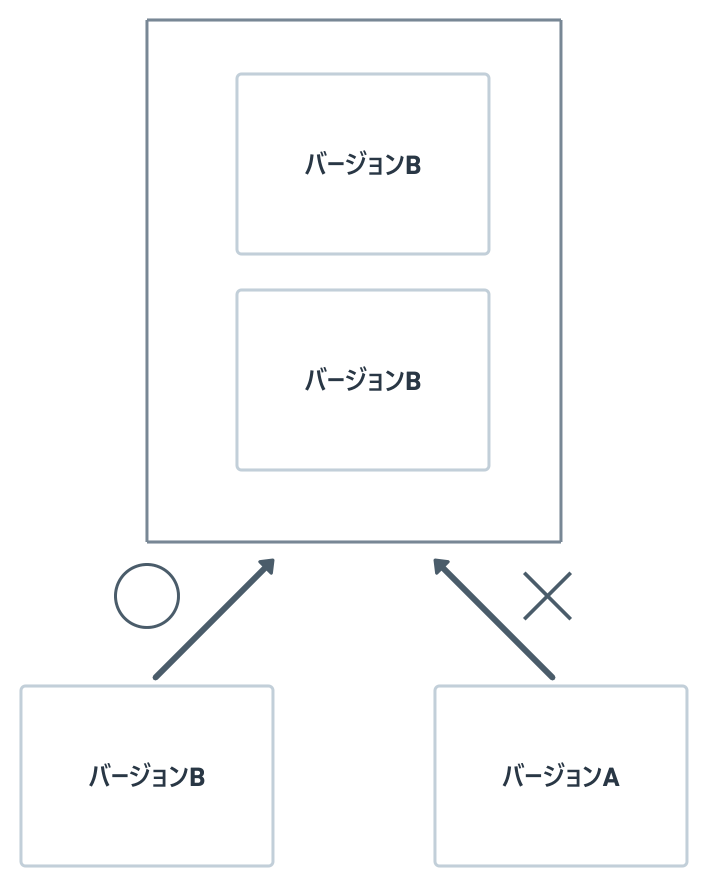
\includegraphics[width=140mm]{sotu/figure/youshi-3.png}
    \caption{Elasticsearchノードのバージョンが異なる場合のクラスタリングの可否}
    \label{4-p16}
  \end{center}
\end{figure}

\begin{figure}[H]
  \begin{center}
    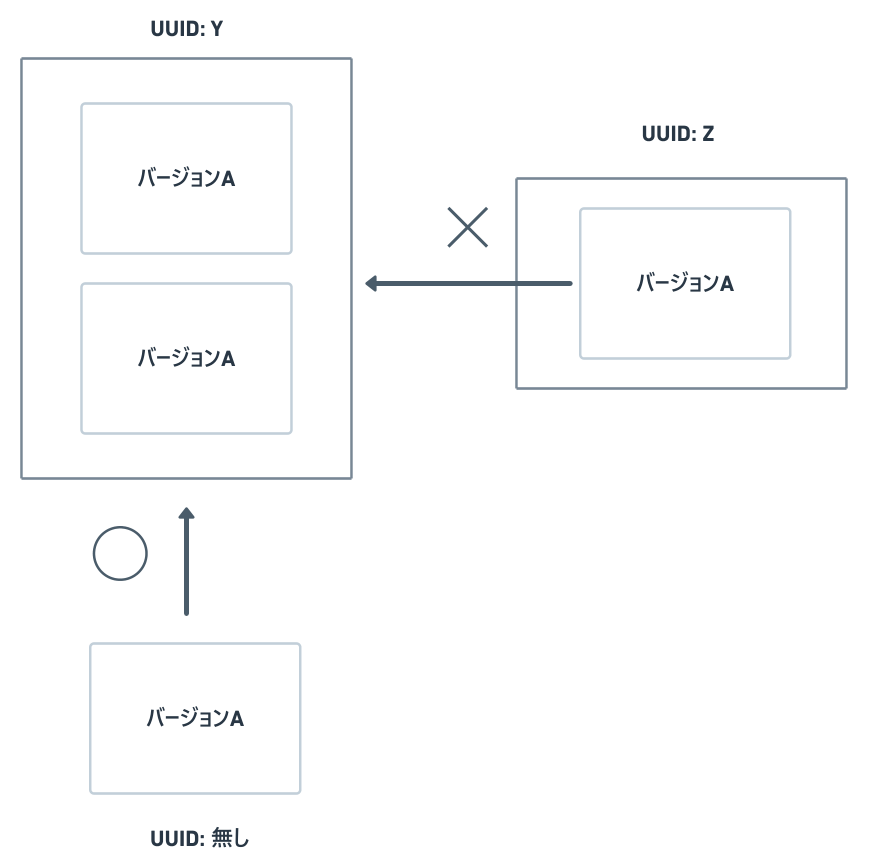
\includegraphics[width=140mm]{sotu/figure/youshi-4.png}
    \caption{UUIDが異なるクラスタにElasticsearchノードを参加させた場合のクラスタリング動作の可否}
    \label{4-p17}
  \end{center}
\end{figure}

次章では結論と今後の課題について述べる.
   % 4章
\chapter{結論と今後の課題}
\label{chap:fifth}

\section{結論}
本研究では, 太陽光発電の計測データ補正とElasticsearchのデータ移行および冗長化について詳細に検討し, 以下の主要な成果を達成した.

% 本研究では, 単一ノードのElasticsearchシステムから学内ゾーン内のクラスタ化システムへデータを移行するプロセスを分析し, さらにサーバゾーンに新しい冗長化されたクラスタ化システムを構築する検証を行った. 

% データ移行プロセスの検証では, CO2データとLEAFの運行日誌に関するデータの移行を行った. CO2データの移行では, 重複データの削除が必要であったが, SQLiteデータベースを用いた手法で対応した. LEAFの運行日誌に関するデータの移行では, 同じ名前のインデックスを移行先のElasticSearchサーバーに作成して, データをインサートすることで行った. 

% サーバーゾーンでのクラスタ構築の検証では, Docker, Docker Composeを使用した事前検証を行った. 異なるバージョンのElasticsearch(7.17.6と7.17.9)を使用したクラスタの構築を試したが, 正常に構築できないことを確認した. 

\begin{itemize}
  \item 相互相関を用いた太陽光発電計測データの時間的ずれの特定手法の提案.
  \item Elasticsearchクラスタへのデータ移行に関する具体的な手順の確立と成功による, データ管理とアクセスの効率化.
  \item サーバーゾーンでのElasticsearchクラスタ構築に向けた仮想環境を使用した事前検証を通じて, バージョンアップの重要性と手順の確立.
\end{itemize}

\section{今後の課題}
本研究の成果を踏まえ, 今後の研究の方向性として以下の課題が考えられる.

\begin{itemize}
  \item 太陽光発電計測データの補正手法のさらなる改善.
  \item 学内ゾーンとサーバーゾーンでそれぞれ稼働しているクラスタごとにKibanaが存在しており, 本研究室で管理するElasticsearchに保存されたデータを一元的に管理, 閲覧することが出来ないので, Kibanaの統合による一元管理の実現.
  % \item Elasticsearchクラスタのセキュリティ対策とデータバックアップ戦略の強化.
  \item システムの継続的なモニタリングと定期的なメンテナンスの実施.
\end{itemize}
   % 結論
\chapter*{謝 辞}
\addcontentsline{toc}{chapter}{謝 辞}

本研究を行うにあたり, 終始, 懇切丁寧な御指導と適切な御助言を賜りました
本学工学部電気電子工学科通信システム工学研究室の都築伸二教授に深甚なる感謝の意を表します.
      % 謝辞
\begin{thebibliography}{99}
%%参考文献の例です。

\bibitem{1}中川清隆,"太陽方位、高度、大気外日射量の計算",\\ http://es.ris.ac.jp/~nakagawa/met\_cal/solar.html, 参照 Feb 13, 2024.
\bibitem{2}Sandia National Laboratories and pvlib python Development Team,"pvlib python",\\ https://pvlib-python.readthedocs.io/en/stable/, 参照 Feb 13, 2024.
\bibitem{3}Elasticsearch B.V., "Install Elasticsearch with Docker | Elasticsearch Guide [7.17] | Elastic",\\ https://www.elastic.co/guide/en/elasticsearch/reference/7.17/docker.html, 参照 Feb 13, 2024.
\bibitem{4}RAKUS Developers Blog, "Dockerとは一体何なんだ?【初心者向け】 - RAKUS Developers Blog | ラクス エンジニアブログ", https://tech-blog.rakus.co.jp/entry/20221007/docker, 参照 Feb 13, 2024.
\end{thebibliography}
      % 参考文献
% \appendix
% \chapter{付録}
%\documentclass[a4j]{jarticle} %ここは関係ない
%\usepackage{listings,jlisting} %日本語のコメントアウトをする場合jlistingが必要
%ここからソースコードの表示に関する設定
%\lstset{
%language = Python,
%basicstyle = \ttfamily\scriptsize,
%  identifierstyle={\small},
%  commentstyle={\smallitshape},
%  keywordstyle={\small\bfseries},
%  ndkeywordstyle={\small},
%  stringstyle={\small\ttfamily},
%  frame={tb},
%  breaklines=true,
%  columns=[l]{fullflexible},
%  numbers=left,
%  xrightmargin=0zw,
%  xleftmargin=0zw,
%  numberstyle={\scriptsize},
%  stepnumber=1,
%  numbersep=1zw,
%  lineskip=-0.5ex
%keywordstyle = {\bfseries \color[cmyk]{0,1,0,0}},
%}
\lstset{
	%プログラム言語(複数の言語に対応,C,C++も可)
 	language = Python,
 	%背景色と透過度
 	%backgroundcolor={\color[gray]{.90}},
 	%枠外に行った時の自動改行
 	breaklines = true,
 	%自動開業後のインデント量(デフォルトでは20[pt])	
 	breakindent = 10pt,
 	%標準の書体
 	basicstyle = \ttfamily\footnotesize,
 	%basicstyle = {\small}
 	%コメントの書体
% 	commentstyle = {\itshape \color[cmyk]{1,0.4,1,0}},
 	%関数名等の色の設定
 	classoffset = 0,
 	%キーワード(int, ifなど)の書体
% 	keywordstyle = {\bfseries \color[cmyk]{0,1,0,0}},
 	%""で囲まれたなどの"文字"の書体
% 	stringstyle = {\ttfamily \color[rgb]{0,0,1}},
 	%枠 "t"は上に線を記載, "T"は上に二重線を記載
	%他オプション:leftline,topline,bottomline,lines,single,shadowbox
% 	frame = TBrl,
	frame = topline,
 	%frameまでの間隔(行番号とプログラムの間)
 	framesep = 5pt,
 	%行番号の位置
 	numbers = left,
	%行番号の間隔
 	stepnumber = 1,
	%右マージン
 	%xrightmargin=0zw,
 	%左マージン
	%xleftmargin=3zw,
	%行番号の書体
 	numberstyle = \tiny,
	%タブの大きさ
 	tabsize = 4,
 	%キャプションの場所("tb"ならば上下両方に記載)
 	captionpos = t
}
%=========================================================================
\section{水源監視システム(送信用Pythonスクリプト)}
\centering
LoRa\_obs\_transmit.pyのソースコードを\ref{loras}に示す.
\begin{lstlisting}[label=loras,caption=LoRa\_obs\_transmit.py]
## +++***coding:utf-8***+++

import time
import os
from datetime import datetime
import serial

""" sleep()をいれて, 少し待たないとエラー落ちする """
time.sleep(60)

class Main() :
    
    def __init__(self):
        """ 初期値および対象ディレクトリの設定 """
        self.s_num = 0

        self.copy_dir = "C:/Users/taikimizukan/Dropbox/sumitomo/obscsv/" 
        self.target_dir = "C:/Users/taikimizukan/Desktop/obs_data/"              
        self.temporary_log = "./temporary_log.txt"

        """ 最終データを取得 """
        with open(self.temporary_log,"r") as f :
            self.old_line = f.readline()
            print("前回のデータ:"+str(self.old_line))
               
        """ 起動時 [$RFINF,ON***]コマンド送信 """
        INF = "$RFINF,ON***"
        with serial.Serial("COM7",115200,timeout=2) as ser :
            time.sleep(2)
            while True :
                for i in INF :
                    ser.write(i.encode("utf-8"))

                result = str(ser.readline())
                if result.find("RESULT,RFINF,ON,OK") > 0 :
                    break
                else :
                    time.sleep(2)

        """ ループ関数実行 """
        self.Loop()
        

    """ 作成日時が最新ファイルのフルパスを取得し返す関数 """
    def get_file_path(self, target_dir) : 
        """ 対象ディレクトリ下の.datファイルのパスを取得し, [target_files]に納める """
        target_files = []
        for root, dir, files in os.walk(target_dir) :
            target_file = [os.path.join(root,f) for f in files if f.endswith(".dat")]# .txt -> .datへ
            target_files.extend(target_file)
        """ 取得した.datファイルのフルパスに作成時間を足してリストに納める """
        file_ctime = []
        for f in target_files :
            file_ctime.append((f,os.path.getctime(f)))        
        """ 取得時間でソートし最新の.datファイルのパスのみ返す"""
        sorted_file_ctime = sorted(file_ctime,key=lambda x :x[1])
                           
        return sorted_file_ctime[len(sorted_file_ctime)-1][0]
        
    """ 最終行を取得, シークエンス番号を加えてコピー """    
    def check_copy(self):
##        name = self.target_file.replace(self.target_dir,"")
        with open(self.target_file,"r") as f :
            """ ファイルデータを全て読み込, 最終行だけを取得 """
            lines = f.readlines()
            if len(lines) > 0 :
                line = lines[len(lines)-1]
            else :
                line = self.old_line
            
        """ 最終行が前回のものと異なるか? """
        if line != self.old_line :
            
            """ シークエンス番号を追加 """
            self.s_num += 1
            
            file_name = line.split(",")
            file_name = "obs_" +"".join(file_name[0:3])
            self.ymd = "".join(file_name[0:3])

            self.old_line = line

            """ Dropboxにコピー """
            with open(self.copy_dir+file_name+".csv","a") as cf :
                data = line.strip() + "," + str(self.s_num)+"\n"
                cf.write(str(data))
            
            """ 最終行を保存 """
            with open(self.temporary_log,"w") as f :
                f.write(line)

            self.arduino_serial(data)
            time.sleep(5)
            self.TxMSG()
            self.Ping()
                    
        else :
            print("Not updated")
            pass

    """ arduinoを経由してLoRaにデータを送信する関数 """
    def arduino_serial(self,d) :
        print("---"*5 + "arduino_serial" + "---"*5)
        buf = 0
        with serial.Serial("COM7",115200,timeout=1) as ser :
            """ ポートを開いて少し待機が必要 """
            time.sleep(2)            
            """ごみの吸出し"""
            buf = ser.readlines()                       
            d = d.strip()
            """ 送信コマンドの形に """
            d = "$RFSND,0004,"+d+"***"
            print("To arduino Data --> " +d)
            
            """ Python(PC) -> arduino -> LoRa だと1文字ずつ送らないといけない? """
            for i in d :
                ser.write(i.encode("utf-8"))                

        """ 0009 : 第二中継機にダミーMSGをとばす, 戻り値を保存 """
    def TxMSG(self) :
        target_add = "0009"
        self.now = datetime.now().strftime("%Y,%m,%d,%H,%M,%S")
        self.today = datetime.today().strftime("%Y%m%d")
        
        msg = "$RFSND,{0},{1},{2},{2}***".format(target_add,self.now,self.counter)

        with serial.Serial("COM7",115200,timeout=15) as ser :
                time.sleep(2)
                for i in msg :
                        ser.write(i.encode("utf-8"))
                        time.sleep(0.05)
                print(ser.readline().decode("utf-8"))
                res = ser.readline().decode("utf-8")

        if len(res) > 10 :
                res = res.replace(" ",",").replace("*",",").replace(":",",")
                with open("C:/Users/taikimizukan/Dropbox/sumitomo/RSSI_CHECK_TX/rssi_tx_obs_{}.csv".format(str(self.today)),"a") as f :
                    f.write(res+"\n")                  
        else :
                pass

    """発電所のLoRaにpingを送って生存確認"""
    def Ping(self) :
        PING = "$RPING,0004***"
        with serial.Serial("COM7",115200,timeout=10) as ser :
            time.sleep(2)
            for i in PING :
                ser.write(i.encode("utf-8"))
                time.sleep(0.05)

            print(ser.readline().decode("utf-8"))
            res_ping = ser.readline().decode("utf-8")
                
        if len(res_ping) > 10 :
            print(res_ping)
            now = datetime.now().strftime("%Y,%m,%d,%H,%M,%S")
            with open("C:/Users/taikimizukan/Dropbox/sumitomo/PING/ping_{}.csv".format(str(self.today)),"a") as f :
                    f.write(str(now)+","+str(self.s_num)+"," + str(res_ping))
        else :
            pass

    """ 繰り返し """
    def Loop(self):  
        while True:
            try :
                time.sleep(20)
                self.target_file = self.get_file_path(self.target_dir)

                self.check_copy()
            
            except Exception as E :
                with open("./Error_Log.txt","a") as ef :
                    ef.write(str(E))


if __name__ == "__main__" :
    Main()
\end{lstlisting}
  % 付録
\end{document}
